% Options for packages loaded elsewhere
\PassOptionsToPackage{unicode}{hyperref}
\PassOptionsToPackage{hyphens}{url}
%
\documentclass[
]{article}
\usepackage{amsmath,amssymb}
\usepackage{lmodern}
\usepackage{iftex}
\ifPDFTeX
  \usepackage[T1]{fontenc}
  \usepackage[utf8]{inputenc}
  \usepackage{textcomp} % provide euro and other symbols
\else % if luatex or xetex
  \usepackage{unicode-math}
  \defaultfontfeatures{Scale=MatchLowercase}
  \defaultfontfeatures[\rmfamily]{Ligatures=TeX,Scale=1}
\fi
% Use upquote if available, for straight quotes in verbatim environments
\IfFileExists{upquote.sty}{\usepackage{upquote}}{}
\IfFileExists{microtype.sty}{% use microtype if available
  \usepackage[]{microtype}
  \UseMicrotypeSet[protrusion]{basicmath} % disable protrusion for tt fonts
}{}
\makeatletter
\@ifundefined{KOMAClassName}{% if non-KOMA class
  \IfFileExists{parskip.sty}{%
    \usepackage{parskip}
  }{% else
    \setlength{\parindent}{0pt}
    \setlength{\parskip}{6pt plus 2pt minus 1pt}}
}{% if KOMA class
  \KOMAoptions{parskip=half}}
\makeatother
\usepackage{xcolor}
\IfFileExists{xurl.sty}{\usepackage{xurl}}{} % add URL line breaks if available
\IfFileExists{bookmark.sty}{\usepackage{bookmark}}{\usepackage{hyperref}}
\hypersetup{
  hidelinks,
  pdfcreator={LaTeX via pandoc}}
\urlstyle{same} % disable monospaced font for URLs
\usepackage[margin=1in]{geometry}
\usepackage{color}
\usepackage{fancyvrb}
\newcommand{\VerbBar}{|}
\newcommand{\VERB}{\Verb[commandchars=\\\{\}]}
\DefineVerbatimEnvironment{Highlighting}{Verbatim}{commandchars=\\\{\}}
% Add ',fontsize=\small' for more characters per line
\usepackage{framed}
\definecolor{shadecolor}{RGB}{248,248,248}
\newenvironment{Shaded}{\begin{snugshade}}{\end{snugshade}}
\newcommand{\AlertTok}[1]{\textcolor[rgb]{0.94,0.16,0.16}{#1}}
\newcommand{\AnnotationTok}[1]{\textcolor[rgb]{0.56,0.35,0.01}{\textbf{\textit{#1}}}}
\newcommand{\AttributeTok}[1]{\textcolor[rgb]{0.77,0.63,0.00}{#1}}
\newcommand{\BaseNTok}[1]{\textcolor[rgb]{0.00,0.00,0.81}{#1}}
\newcommand{\BuiltInTok}[1]{#1}
\newcommand{\CharTok}[1]{\textcolor[rgb]{0.31,0.60,0.02}{#1}}
\newcommand{\CommentTok}[1]{\textcolor[rgb]{0.56,0.35,0.01}{\textit{#1}}}
\newcommand{\CommentVarTok}[1]{\textcolor[rgb]{0.56,0.35,0.01}{\textbf{\textit{#1}}}}
\newcommand{\ConstantTok}[1]{\textcolor[rgb]{0.00,0.00,0.00}{#1}}
\newcommand{\ControlFlowTok}[1]{\textcolor[rgb]{0.13,0.29,0.53}{\textbf{#1}}}
\newcommand{\DataTypeTok}[1]{\textcolor[rgb]{0.13,0.29,0.53}{#1}}
\newcommand{\DecValTok}[1]{\textcolor[rgb]{0.00,0.00,0.81}{#1}}
\newcommand{\DocumentationTok}[1]{\textcolor[rgb]{0.56,0.35,0.01}{\textbf{\textit{#1}}}}
\newcommand{\ErrorTok}[1]{\textcolor[rgb]{0.64,0.00,0.00}{\textbf{#1}}}
\newcommand{\ExtensionTok}[1]{#1}
\newcommand{\FloatTok}[1]{\textcolor[rgb]{0.00,0.00,0.81}{#1}}
\newcommand{\FunctionTok}[1]{\textcolor[rgb]{0.00,0.00,0.00}{#1}}
\newcommand{\ImportTok}[1]{#1}
\newcommand{\InformationTok}[1]{\textcolor[rgb]{0.56,0.35,0.01}{\textbf{\textit{#1}}}}
\newcommand{\KeywordTok}[1]{\textcolor[rgb]{0.13,0.29,0.53}{\textbf{#1}}}
\newcommand{\NormalTok}[1]{#1}
\newcommand{\OperatorTok}[1]{\textcolor[rgb]{0.81,0.36,0.00}{\textbf{#1}}}
\newcommand{\OtherTok}[1]{\textcolor[rgb]{0.56,0.35,0.01}{#1}}
\newcommand{\PreprocessorTok}[1]{\textcolor[rgb]{0.56,0.35,0.01}{\textit{#1}}}
\newcommand{\RegionMarkerTok}[1]{#1}
\newcommand{\SpecialCharTok}[1]{\textcolor[rgb]{0.00,0.00,0.00}{#1}}
\newcommand{\SpecialStringTok}[1]{\textcolor[rgb]{0.31,0.60,0.02}{#1}}
\newcommand{\StringTok}[1]{\textcolor[rgb]{0.31,0.60,0.02}{#1}}
\newcommand{\VariableTok}[1]{\textcolor[rgb]{0.00,0.00,0.00}{#1}}
\newcommand{\VerbatimStringTok}[1]{\textcolor[rgb]{0.31,0.60,0.02}{#1}}
\newcommand{\WarningTok}[1]{\textcolor[rgb]{0.56,0.35,0.01}{\textbf{\textit{#1}}}}
\usepackage{graphicx}
\makeatletter
\def\maxwidth{\ifdim\Gin@nat@width>\linewidth\linewidth\else\Gin@nat@width\fi}
\def\maxheight{\ifdim\Gin@nat@height>\textheight\textheight\else\Gin@nat@height\fi}
\makeatother
% Scale images if necessary, so that they will not overflow the page
% margins by default, and it is still possible to overwrite the defaults
% using explicit options in \includegraphics[width, height, ...]{}
\setkeys{Gin}{width=\maxwidth,height=\maxheight,keepaspectratio}
% Set default figure placement to htbp
\makeatletter
\def\fps@figure{htbp}
\makeatother
\setlength{\emergencystretch}{3em} % prevent overfull lines
\providecommand{\tightlist}{%
  \setlength{\itemsep}{0pt}\setlength{\parskip}{0pt}}
\setcounter{secnumdepth}{-\maxdimen} % remove section numbering
\ifLuaTeX
  \usepackage{selnolig}  % disable illegal ligatures
\fi

\author{}
\date{\vspace{-2.5em}}

\begin{document}

{
\setcounter{tocdepth}{2}
\tableofcontents
}
\hypertarget{resumen}{%
\section{Resumen}\label{resumen}}

Esta guía \footnote{Puede consultar Holland (1986), Angrist y Pischke
  Angrist, Joshua y Jörn-Steffen Pischke. 2008. Mostly Harmless
  Econometrics: An Empiricist's Companion. Princeton University Press.}
presenta una discusión más formal de la independencia y de los supuestos
necesarios para estimar los efectos causales. Además, describe diez
tipos distintos de efectos causales en los que podríamos estar
interesados. Como demostramos en nuestra guía de inferencia causal, la
aleatorización simple permite producir estimaciones del promedio de los
efectos causales al nivel de la unidad en una muestra. Este efecto
causal promedio o efecto promedio del tratamiento (Average Treatment
Effect, ATE) es un concepto poderoso porque provee una solución al
problema de no poder observar todos los contrafactuales relevantes para
la estimación. Sin embargo, no es la unica forma de abordar este
problema. De hecho, hay muchas cantidades de interés causal diferentes.
El objetivo de esta guía es ayudarlo a elegir estimandos (un parámetro
de interés) y estimadores (procedimientos para calcular estimaciones de
esos parámetros) que sean apropiados y significativos para sus datos.

\hypertarget{efecto-promedio-del-tratamiento}{%
\section{1 Efecto promedio del
tratamiento}\label{efecto-promedio-del-tratamiento}}

Comenzamos revisando cómo, con la aleatorización, una simple diferencia
de medias proporciona una estimación no sesgada del ATE. A continuación,
presentamos algunos conceptos estadísticos comunes y la notación que
utilizamos a lo largo de esta guía.

Primero definimos el efecto del tratamiento para una observación
individual (una persona, hogar, ciudad, etc.) como la diferencia entre
el comportamiento de esa unidad bajo tratamiento \((Y_ {i} (1))\) y
control \[\tau_{i}=Y_{i}(1)-Y_{i}(0)\] Dado que solo podemos observar
\$Y\_\{i\}(1) \$ o \(Y_ {i} (0)\), no tenemos forma de saber cuál es el
efecto del tratamiento individual. Ahora sea \(D_{i}\) un indicador de
si una observación está en el grupo de tratamiento o control. Si el
tratamiento se asigna al azar, \(D_ {i}\) es independiente, no solo de
los resultados potenciales sino también de cualquier covariable
(observada y no observada) que pueda predecir también esos resultados
\(((Y_ {i} (1), Y_ {i } (0),X_ {i} \perp \perp D_ {i}))\) \footnote{Ver
  Holland, Angrist y Pischke para una discusión más formal sobre la
  independencia y los supuestos necesarios para estimar los efectos
  causales.}.

Suponga que nuestro diseño tiene \(m\) unidades en el grupo de
tratamiento y \(N - m\) en el de control. Supongamos que reasignamos
repetidamente el tratamiento al azar muchas veces y cada vez calculamos
la diferencia de medias entre los grupos de tratamiento y de control y
luego registramos este valor en una lista. El promedio de los valores en
esa lista será el mismo que la diferencia de los promedios de los
resultados potenciales reales si hubiéramos observado todos los
resultados potenciales posibles para todas las observaciones
\footnote{Es decir, \((E(Y_i(1)|D=1)=E(Y_i(1)|D=0)=E(Y_i(1)))\) and
  \((E(Y_i(0)|D=1)=E(Y_i(0)|D=0)=E(Y_i(0)))\)}. Otra forma de expresar
esta característica del efecto promedio del tratamiento y el estimador
del mismo es decir que la diferencia de medias observadas es un
estimador insesgado del efecto del tratamiento causal promedio.

\[ATE\equiv\frac{1}{N}\sum^{N}_{i=1}\tau_{i}=\frac{\sum^{N}_{1}Y_{i}(1)}{N}-\frac{\sum^{N}_{1}Y_{i}(0)}{N}\]

A menudo estimamos el ATE utilizando la diferencia de medias observada:
\footnote{Las estimaciones a menudo se escriben con un acento
  (\(\widehat {ATE}\)) para reflejar la diferencia entre la estimación
  de nuestra muestra particular y el estimando, es decir la cantidad
  objetivo de nuestra estimación que no podemos observar. A menos que se
  indique lo contrario, en esta guía nos enfocamos en generar
  estimaciones a partir de la muestra y posteriormente omitimos esta
  notación explícita. Ver Gerber y Green (2012) para una introducción
  concisa a esta distinción e Imbens y Wooldridge (2007) para una
  revisión completa de estos conceptos.}

\[\widehat{ATE} =\frac{\sum^m_1Z_{i}Y_{i}}{m}-\frac{\sum^{N}_{m+1}(1-Z_{i})Y_{i}}{N-m}\]

La inferencia estadística sobre el ATE estimado requiere que sepamos
cómo este variaría entre cada aleatorización. Para eso podemos escribir
la varianza entre aleatorizaciones de la siguiente manera:

\[V(ATE) = \frac{N}{N-1} [\frac{V(Y_{i}(1))}{m}+\frac{V(Y_{i}(0))}{N-m}]-\frac{1}{N-1}[V(Y_{i}(1))+V(Y_{i}(0))-2Cov(Y_{i}(1),Y_{i}(0))]\]

y estimar esta cantidad a partir de las estimaciones muestrales de la
varianza en cada grupo. \footnote{La covarianza de
  \(Y_{i} (1), Y_ {i} (0)\) es imposible de observar, pero el estimador
  ``Neyman'' de la varianza que omite el término de covarianza
  proporciona una estimación conservadora (demasiado grande) de la
  varianza muestral verdadera porque tendemos a suponer que la
  covarianza es positiva. Dado que en general nos preocupa minimizar la
  tasa de error de tipo I (rechazando incorrectamente la hipótesis nula
  verdadera), preferimos utilizar estimaciones conservadoras de la
  varianza. Ver también Dunning (2010) y Gerber y Green (2012) para la
  justificación del estimador de varianza conservador.}

Un modelo lineal que regresa el resultado observado \(Y_ {i}\) en un
indicador de la asignación del tratamiento \(D_{i}\) nos sirve como
estimador del ATE (y con algunos ajustes adicionales de la varianza del
ATE):

\[Y_{i}=Y_{i}(0)(1-D_{i})+Y_{i}(1)D_{i}=\beta_{0}+\beta_{1}D_{i}+u\] ya
que podemos reorganizar los términos de modo que \(\beta_{0}\) estime el
promedio entre las observaciones de control \((Y_ {i} (0) ∣D_ {i} = 0)\)
y \(\beta_{1}\) estime las diferencias de las medias
\((Y_ {i} (1) ∣D_ {i} = 1) - (Y_ {i} (1) ∣D_ {i} = 0)\). En el siguiente
código, creamos una muestra de 1000 observaciones y asignamos
aleatoriamente un tratamiento \(D_i\) con un efecto constante para la
mitad de las unidades. Estimamos el ATE utilizando la regresión de
mínimos cuadrados ordinarios (MCO) para calcular la diferencia de medias
observada. El cálculo de las medias en cada grupo y su diferencia
también produciría una estimación no sesgada del ATE. Tenga en cuenta
que el ATE estimado del estimador de MCO es insesgado porque suponemos
que los errores en este modelo lineal son independientes y están
distribuidos de manera idéntica. Cuando nuestro tratamiento afecta tanto
al valor promedio del resultado como a la distribución de las
respuestas, esta supuesto ya no se cumple y necesitamos ajustar los
errores estándar de MCO utilizando un estimador sándwich de Huber-White
para obtener las estimaciones correctas (basadas en la varianza de el
ATE) para hacer inferencia estadística. \footnote{Lin (2013)}
Finalmente, través de la simulación demostramos que estos estimadores
son insesgados.

\begin{Shaded}
\begin{Highlighting}[]
\FunctionTok{set.seed}\NormalTok{(}\DecValTok{1234}\NormalTok{) }\CommentTok{\# Por replicabilidad }
\NormalTok{N }\OtherTok{=} \DecValTok{1000} \CommentTok{\# Tamaño de la población}
\NormalTok{Y0 }\OtherTok{=} \FunctionTok{runif}\NormalTok{(N) }\CommentTok{\# Resultado potencial bajo la condición de control}
\NormalTok{Y1 }\OtherTok{=}\NormalTok{ Y0 }\SpecialCharTok{+} \DecValTok{1} \CommentTok{\# Resultado potencial bajo la condición de tratamiento}
\NormalTok{D }\OtherTok{=} \FunctionTok{sample}\NormalTok{((}\DecValTok{1}\SpecialCharTok{:}\NormalTok{N)}\SpecialCharTok{\%\%}\DecValTok{2}\NormalTok{) }\CommentTok{\#igual a 1 si la unidad es tratada, 0 de lo contrario}
\NormalTok{Y }\OtherTok{=}\NormalTok{ D}\SpecialCharTok{*}\NormalTok{Y1 }\SpecialCharTok{+}\NormalTok{ (}\DecValTok{1}\SpecialCharTok{{-}}\NormalTok{D)}\SpecialCharTok{*}\NormalTok{Y0 }\CommentTok{\# Variable de resultado de la población}
\NormalTok{samp }\OtherTok{=} \FunctionTok{data.frame}\NormalTok{(D,Y) }

\NormalTok{ATE }\OtherTok{=} \FunctionTok{coef}\NormalTok{(}\FunctionTok{lm}\NormalTok{(Y}\SpecialCharTok{\textasciitilde{}}\NormalTok{D,}\AttributeTok{data=}\NormalTok{samp))[}\DecValTok{2}\NormalTok{] }\CommentTok{\#lo mismo que with(samp,mean(Y[Z==1]){-}mean(Y[Z==0])) }

\CommentTok{\# ATE de la muestra (SATE) con error estándar Neyman }
\CommentTok{\# o justificados en la aleatorización}
\CommentTok{\# que son iguales al error estándar del MCO cuando no hay covariables o bloques}
\FunctionTok{library}\NormalTok{(lmtest) }
\FunctionTok{library}\NormalTok{(sandwich) }
\NormalTok{fit}\OtherTok{\textless{}{-}}\FunctionTok{lm}\NormalTok{(Y}\SpecialCharTok{\textasciitilde{}}\NormalTok{D,}\AttributeTok{data=}\NormalTok{samp) }
\FunctionTok{coef}\NormalTok{(}\FunctionTok{summary}\NormalTok{(fit))[}\StringTok{"D"}\NormalTok{,}\DecValTok{1}\SpecialCharTok{:}\DecValTok{2}\NormalTok{]}
\end{Highlighting}
\end{Shaded}

\begin{verbatim}
##   Estimate Std. Error 
## 1.01820525 0.01841784
\end{verbatim}

\begin{Shaded}
\begin{Highlighting}[]
\NormalTok{ATE.se}\OtherTok{\textless{}{-}}\FunctionTok{coeftest}\NormalTok{(fit,}\FunctionTok{vcovHC}\NormalTok{(fit,}\AttributeTok{type=}\StringTok{"HC2"}\NormalTok{))[}\StringTok{"D"}\NormalTok{,}\DecValTok{2}\NormalTok{] }
 \CommentTok{\#lo mismo que with(samp,sqrt(var(Y[D==1])/sum(D)+var(Y[D==0])/(n{-}sum(D))) }

\CommentTok{\# Evaluar si no hay sesgo y simular el error estándar}
\NormalTok{getATE}\OtherTok{\textless{}{-}}\ControlFlowTok{function}\NormalTok{() \{}
\NormalTok{  D }\OtherTok{=} \FunctionTok{sample}\NormalTok{((}\DecValTok{1}\SpecialCharTok{:}\NormalTok{N)}\SpecialCharTok{\%\%}\DecValTok{2}\NormalTok{) }\CommentTok{\#  igual a 1 si la unidad es tratada, 0 de lo contrario}
\NormalTok{  Y }\OtherTok{=}\NormalTok{ D}\SpecialCharTok{*}\NormalTok{Y1 }\SpecialCharTok{+}\NormalTok{ (}\DecValTok{1}\SpecialCharTok{{-}}\NormalTok{D)}\SpecialCharTok{*}\NormalTok{Y0 }
  \FunctionTok{coef}\NormalTok{(}\FunctionTok{lm}\NormalTok{(Y}\SpecialCharTok{\textasciitilde{}}\NormalTok{D))[[}\StringTok{"D"}\NormalTok{]] }
\NormalTok{\} }

\NormalTok{manyATEs}\OtherTok{\textless{}{-}}\FunctionTok{replicate}\NormalTok{(}\DecValTok{10000}\NormalTok{,}\FunctionTok{getATE}\NormalTok{()) }

\DocumentationTok{\#\# Sesgo}
\FunctionTok{c}\NormalTok{(}\AttributeTok{ATE=}\FunctionTok{mean}\NormalTok{(Y1)}\SpecialCharTok{{-}}\FunctionTok{mean}\NormalTok{(Y0), }\AttributeTok{ExpEstATE=}\FunctionTok{mean}\NormalTok{(manyATEs)) }
\end{Highlighting}
\end{Shaded}

\begin{verbatim}
##       ATE ExpEstATE 
## 1.0000000 0.9999077
\end{verbatim}

\begin{Shaded}
\begin{Highlighting}[]
\DocumentationTok{\#\# Error estándar}
\DocumentationTok{\#\#\# Fórmula del error estándar real}
\NormalTok{V}\OtherTok{\textless{}{-}}\FunctionTok{var}\NormalTok{(}\FunctionTok{cbind}\NormalTok{(Y0,Y1)) }
\NormalTok{varc}\OtherTok{\textless{}{-}}\NormalTok{V[}\DecValTok{1}\NormalTok{,}\DecValTok{1}\NormalTok{] }
\NormalTok{vart}\OtherTok{\textless{}{-}}\NormalTok{V[}\DecValTok{2}\NormalTok{,}\DecValTok{2}\NormalTok{] }
\NormalTok{covtc}\OtherTok{\textless{}{-}}\NormalTok{V[}\DecValTok{1}\NormalTok{,}\DecValTok{2}\NormalTok{] }
\NormalTok{n}\OtherTok{\textless{}{-}}\FunctionTok{sum}\NormalTok{(D) }
\NormalTok{m}\OtherTok{\textless{}{-}}\NormalTok{N}\SpecialCharTok{{-}}\NormalTok{n }
\NormalTok{varestATE}\OtherTok{\textless{}{-}}\NormalTok{((N}\SpecialCharTok{{-}}\NormalTok{n)}\SpecialCharTok{/}\NormalTok{(N}\DecValTok{{-}1}\NormalTok{))}\SpecialCharTok{*}\NormalTok{(vart}\SpecialCharTok{/}\NormalTok{n) }\SpecialCharTok{+}\NormalTok{ ((N}\SpecialCharTok{{-}}\NormalTok{m)}\SpecialCharTok{/}\NormalTok{(N}\DecValTok{{-}1}\NormalTok{))}\SpecialCharTok{*}\NormalTok{ (varc}\SpecialCharTok{/}\NormalTok{m) }\SpecialCharTok{+}\NormalTok{ (}\DecValTok{2}\SpecialCharTok{/}\NormalTok{(N}\DecValTok{{-}1}\NormalTok{)) }\SpecialCharTok{*}\NormalTok{ covtc }

\DocumentationTok{\#\#\# Compararar errores estándar }
\FunctionTok{c}\NormalTok{(}\AttributeTok{SimulatedSE=} \FunctionTok{sd}\NormalTok{(manyATEs), }\AttributeTok{TrueSE=}\FunctionTok{sqrt}\NormalTok{(varestATE), }\AttributeTok{ConservativeSE=}\NormalTok{ATE.se) }
\end{Highlighting}
\end{Shaded}

\begin{verbatim}
##    SimulatedSE         TrueSE ConservativeSE 
##     0.01835497     0.01842684     0.01841784
\end{verbatim}

\hypertarget{efecto-condicional-promedio-del-tratamiento}{%
\section{2 Efecto condicional promedio del
tratamiento}\label{efecto-condicional-promedio-del-tratamiento}}

El problema de enfocarse únicamente el efecto promedio del tratamiento
es que desvía la atención del hecho de que los efectos del tratamiento
pueden ser muy diferentes para diferentes tipos de personas. Si bien el
``problema fundamental de la inferencia causal'' sugiere que medir los
efectos causales para unidades individuales es imposible, hacer
inferencias sobre grupos de unidades no lo es.

La asignación aleatoria asegura que el tratamiento sea independiente de
las variables de resultado y de cualquier covariable (observada y no
observada). Sin embargo, a veces tenemos información adicional sobre las
unidades experimentales tal como eran antes de que se realizara el
experimento. Denotaremos esta información como \(X_{i}\). \(X_{i}\)
puede ayudarnos a comprender cómo los efectos del tratamiento varían
entre los subgrupos. Por ejemplo, podemos sospechar que los hombres y
las mujeres responden de manera diferente al tratamiento, y podemos
probar esta hetorogeneidad estimando el ATE condicional para cada
subgrupo por separado
\((CATE = E (Y_{i} (1) -Y_{i} (0)∣D_ {i}, X_{i}))\). Si nuestra
covariable es continua podemos probar sus efectos moderadores
interactuando la variable continua con el tratamiento. Sin embargo,
tenga en cuenta que el efecto del tratamiento ahora está condicionado
tanto al estado del tratamiento como al valor de la variable
condicionante en la que se evalúa el efecto, por lo que debemos ajustar
nuestra interpretación y los errores estándar en
consecuencia.{[}\^{}7{]}

Una advertencia: enfocarse en los efectos del tratamiento en las
dimensiones que se ven afectadas por el tratamiento es peligroso y puede
conducir a inferencias incorrectas. Por ejemplo, si quisiera ver cómo la
administración de un medicamento produce mejoras en la salud, podría
buscar por separado a hombres y mujeres, pero no podría buscar por
separado a los que tomaron el medicamento y a los que no (este es un
ejemplo de inferencia para que los que cumplen con la asignación al
tramiento y este tipo de inferencia requiere otras técnicas descritas en
el punto 4).

\hypertarget{efectos-de-la-intenciuxf3n-de-tratar}{%
\section{3 Efectos de la intención de
tratar}\label{efectos-de-la-intenciuxf3n-de-tratar}}

Fuera de un entorno de laboratorio controlado, los sujetos que asignamos
al tratamiento a menudo no son los mismos que los sujetos que realmente
reciben el tratamiento. Cuando algunos sujetos asignados al tratamiento
no lo reciben, lo llamamos un experimento con incumplimiento unilateral.
Cuando además, algunos sujetos asignados al control también reciben el
tratamiento, decimos que hay un incumplimiento bilateral. Por ejemplo,
en un experimento para promover la votación electoral, es posible que
algunas sujetos asignados para recibir una carta no lo reciban. Quizás
hayan cambiado de dirección o nunca hayan revisado su correo. De manera
similar, algunas observaciones asignadas al control pueden recibir el
tratamiento. Quizás se acaban de mudar y el correo del inquilino
anterior todavía llega a ese domicilio.

Cuando hay incumplimiento, la recepción del tratamiento ya no es
independiente de las variable resultados y posibles factores que puedan
generar distorsión. Las personas que realmente leen su correo
probablemente difieran en varias formas de las personas que tiran su
correo (o leen el correo ajeno) y estas diferencias probablemente
también afecten su probabilidad de votar. La diferencia de medias entre
los sujetos asignados al tratamiento y al control ya no estima el ATE,
sino que estima lo que se llama un efecto por intención de tratar
(Intention to treat, ITT). A menudo interpretamos el ITT como el efecto
de darle a alguien la oportunidad de recibir el tratamiento. El ITT es
particularmente relevante para evaluar programas e intervenciones con
participación voluntaria.

En el siguiente código, generamos datos con incumplimiento unilateral.
Aunque el verdadero efecto del tratamiento para las personas que
realmente recibieron el tratamiento es 2, nuestro ITT estimado es menor
(aproximadamente 1) porque solo algunas de las personas asignadas al
tratamiento realmente lo reciben.

\begin{Shaded}
\begin{Highlighting}[]
\FunctionTok{set.seed}\NormalTok{(}\DecValTok{1234}\NormalTok{) }\CommentTok{\# Por replicabilidad}
\NormalTok{n }\OtherTok{=} \DecValTok{1000} \CommentTok{\# Tamaño de la población}
\NormalTok{Y0 }\OtherTok{=} \FunctionTok{runif}\NormalTok{(n) }\CommentTok{\# Resultado potencial bajo el control}
\NormalTok{C }\OtherTok{=} \FunctionTok{sample}\NormalTok{((}\DecValTok{1}\SpecialCharTok{:}\NormalTok{n)}\SpecialCharTok{\%\%}\DecValTok{2}\NormalTok{) }\CommentTok{\# Si el sujeto cumple con la asignación}
\NormalTok{Y1 }\OtherTok{=}\NormalTok{ Y0 }\SpecialCharTok{+} \DecValTok{1} \SpecialCharTok{+}\NormalTok{C }\CommentTok{\# Resultado potencial bajo el tratamiento }
\NormalTok{Z }\OtherTok{=} \FunctionTok{sample}\NormalTok{((}\DecValTok{1}\SpecialCharTok{:}\NormalTok{n)}\SpecialCharTok{\%\%}\DecValTok{2}\NormalTok{) }\CommentTok{\# Asignación al tratamiento}
\NormalTok{D }\OtherTok{=}\NormalTok{ Z}\SpecialCharTok{*}\NormalTok{C }\CommentTok{\# Indicador de si recibe el tratamiento}
\NormalTok{Y }\OtherTok{=}\NormalTok{ D}\SpecialCharTok{*}\NormalTok{Y1 }\SpecialCharTok{+}\NormalTok{ (}\DecValTok{1}\SpecialCharTok{{-}}\NormalTok{D)}\SpecialCharTok{*}\NormalTok{Y0 }\CommentTok{\# Variable de resultado}
\NormalTok{samp }\OtherTok{=} \FunctionTok{data.frame}\NormalTok{(Z,Y)}
\NormalTok{ITT}\OtherTok{\textless{}{-}}\FunctionTok{coef}\NormalTok{(}\FunctionTok{lm}\NormalTok{(Y}\SpecialCharTok{\textasciitilde{}}\NormalTok{Z,}\AttributeTok{data=}\NormalTok{samp))[}\DecValTok{2}\NormalTok{]}
\end{Highlighting}
\end{Shaded}

\hypertarget{efectos-de-tratamiento-promedio-para-los-que-cumplen}{%
\section{4 Efectos de tratamiento promedio para los que
cumplen}\label{efectos-de-tratamiento-promedio-para-los-que-cumplen}}

¿Qué pasa si estamos interesado en averiguar los efectos de un
tratamiento en aquellas personas que realmente recibieron el tratamiento
y no solo en aquellas personas a las que se les asignó el tratamiento?
Por ejemplo, ¿cuál es el efecto de los anuncios de radio en el
comportamiento de voto de las personas que realmente escuchan los
anuncios?

Esto resulta ser un problema difícil de abordar (en esta guía puede
encontrar más información al respecto). Las razones del incumplimiento
del tratamiento pueden ser una variable omitida. Si bien la recepción
del tratamiento ya no es independiente de los posibles resultados, la
asignación del estado del tratamiento sí lo es. Siempre que la
asignación aleatoria tenga algún efecto positivo sobre la probabilidad
de recibir tratamiento, podemos usarlo como un instrumento para
identificar los efectos del tratamiento en la subpoblación de sujetos
que cumplen con la asignación al tratamiento.

Siguiendo la notación de Angrist y Pischke \footnote{Angrist, Joshua y
  Jörn-Steffen Pischke. 2008. Mostly Harmless Econometrics: An
  Empiricist's Companion. Princeton university press.}, sea \(Z\) un
indicador de si se asignó una observación al tratamiento y \(D_{i}\)
indica si ese sujeto realmente recibió el tratamiento. Los experimentos
con incumplimiento están compuestos por personas que siempre toman el
tratamiento (\(D_{i} = 1\), independientemente de \$
Z\_\{i\}\(), personas que nunca lo toman (\)D\_ \{i\} = 0\$
independientemente de \(Z_ {i}\)) y los que cumplen con la asignación
(\(D_ {i} = 1\) cuando \$Z\_\{i\} = 1 \$ y \(0\) cuando
\(Z_ {i} = 0\)).\footnote{Por lo general, asumimos monotonicidad, lo que
  significa que no hay quienes desobedecen o desafían la asignación o
  personas que solo toman el tratamiento cuando se les asigna el control
  (\(D_{i} = 1\) cuando \(Z_i = 0\) ) y rechazan el tratamiento cuando
  se les asigna al tratamiento.} Podemos estimar un efecto causal
promedio del cumplidor (Complier Average Causal Effect, CACE), a veces
también llamado efecto de tratamiento promedio local (LATE, Local
Average Treatment Effect), al ponderar el ITT (el efecto de \(Z\) en
\(Y\)) por la efectividad de la asignación aleatoria en la aceptación
del tratamiento (el efecto de \(Z\) en \$ D\$)

\[CACE= \frac{Effect of Z on Y}{Effect of Z on D}=\frac{E(Y_i∣Z_i=1)-E(Y_i|Z_i=0)}{E(D_i|Z_i=1)-E(D_i|Z_i=0)}\]

El estimador anterior destaca el hecho de que el ITT y el CACE convergen
a medida que nos acercamos a un cumplimiento total. Construir errores
estándar para fracciones es algo engorroso, por lo que generalmente
estimamos un CACE usando regresión de mínimos cuadrados de dos etapas
con asignación aleatoria, \(Z_i\), que sirve como instrumento para la
recepción del tratamiento \(D_i\) en la primera etapa del modelo. Este
enfoque simplifica la estimación de errores estándar y permite la
inclusión de covariables como instrumentos adicionales. Presentamos
ambas estrategias en el siguiente código utilizando datos con
incumplimiento bilateral. Sin embargo, tenga en cuenta que cuando los
instrumentos son débiles (por ejemplo, la asignación aleatoria tuvo solo
un efecto pequeño en la recepción del tratamiento), los estimadores de
variables instrumentales y sus errores estándar pueden ser sesgados e
inconsistentes \footnote{Angrist, Joshua, and Jörn-Steffen Pischke.
  2008. Mostly Harmless Econometrics: An Empiricist's Companion.
  Princeton university press.; Bound, Jaeger, and Baker (1995)}.

\begin{Shaded}
\begin{Highlighting}[]
\FunctionTok{set.seed}\NormalTok{(}\DecValTok{1234}\NormalTok{) }\CommentTok{\# Por replicabilidad}
\NormalTok{n }\OtherTok{=} \DecValTok{1000} \CommentTok{\# Tamaño de la población}
\NormalTok{Y0 }\OtherTok{=} \FunctionTok{runif}\NormalTok{(n) }\CommentTok{\# Resultado potencial bajo el control}
\NormalTok{Y1 }\OtherTok{=}\NormalTok{ Y0 }\SpecialCharTok{+} \DecValTok{1} \CommentTok{\# Resultado potencial bajo el tratamiento }
\NormalTok{Z }\OtherTok{=} \FunctionTok{sample}\NormalTok{((}\DecValTok{1}\SpecialCharTok{:}\NormalTok{n)}\SpecialCharTok{\%\%}\DecValTok{2}\NormalTok{) }\CommentTok{\# Asignación al tratamiento}
\NormalTok{pD}\OtherTok{\textless{}{-}}\FunctionTok{pnorm}\NormalTok{(}\SpecialCharTok{{-}}\DecValTok{1}\SpecialCharTok{+}\FunctionTok{rnorm}\NormalTok{(n,}\AttributeTok{mean=}\DecValTok{2}\SpecialCharTok{*}\NormalTok{Z)) }\CommentTok{\# Incumplimiento}
\NormalTok{D}\OtherTok{\textless{}{-}}\FunctionTok{rbinom}\NormalTok{(n,}\DecValTok{1}\NormalTok{,pD) }\CommentTok{\# Recepción del tratamiento sin incumplimiento}
\NormalTok{Y }\OtherTok{=}\NormalTok{ D}\SpecialCharTok{*}\NormalTok{Y1 }\SpecialCharTok{+}\NormalTok{ (}\DecValTok{1}\SpecialCharTok{{-}}\NormalTok{D)}\SpecialCharTok{*}\NormalTok{Y0 }\CommentTok{\# Variable de resultado}
\NormalTok{samp }\OtherTok{=} \FunctionTok{data.frame}\NormalTok{(Z,D,Y) }

\CommentTok{\# IV estimate library(AER) CACE = coef(ivreg(Y \textasciitilde{} D | Z, data = samp))[2] }

\CommentTok{\# Wald Estimator ITT\textless{}{-}coef(lm(Y\textasciitilde{}Z,data=samp))[2] ITT.D\textless{}{-}coef(lm(D\textasciitilde{}Z,data=samp))[2] CACE.wald\textless{}{-}ITT/ITT.D}
\end{Highlighting}
\end{Shaded}

\hypertarget{efectos-promedio-del-tratamiento-en-la-poblaciuxf3n-y-la-muestra}{%
\section{5 Efectos promedio del tratamiento en la población y la
muestra}\label{efectos-promedio-del-tratamiento-en-la-poblaciuxf3n-y-la-muestra}}

A menudo queremos hacer generalizaciones a partir de nuestra muestra
para poder hacer afirmaciones sobre una población de interés más amplia
\footnote{Vea Imai, King y Stuart (2008) para una revisión más detallada
  de los temas discutidos en esta sección.}. Sea \(S_i\) un indicador de
si un sujeto está en nuestra muestra. El efecto de tratamiento promedio
de la muestra (Sample Average Treatment Effect, SATE) se define
simplemente como \(E(Y_i (1) -Y_i(0) | S_i = 1)\) y la población
\(E(Y_i (1) -Y_i (0))\). Con una muestra aleatoria grande de una
población bien definida y con cumplimiento total de la asignación al
tratamiento, el SATE y el PATE (ATE de la población) son iguales en
expectativa y, por lo tanto, una buena estimación para uno (como una
diferencia de medias muestrales) será una buena estimación para el otro.
\footnote{Imbens, Guido y Jeffrey M Wooldridge. 2007. What's New in
  Econometrics? NBER.}

En la práctica, el grupo experimental puede consistir de un grupo de
unidades seleccionadas de una manera desconocida de una población
vagamente definida de tales unidades y el cumplimiento de la asignación
de tratamiento puede ser menos que completo. En tales casos, nuestro
SATE puede diferir del PATE y utilizar uno para estimar el otro se
vuelve más complicado. Imai, King y Stuart (2008) descomponen la
diferencia entre estas estimaciones en un error que surge de la
selección de la muestra y el imbalance del tratamiento. El error de la
selección de la muestra surge de diferentes distribuciones de
covariables (observadas y no observadas) en nuestra muestra y población.
Por ejemplo, las personas en un ensayo médico a menudo difieren de la
población para la que estaría disponible el medicamento. El error de
imbalance del tratamiento refleja las diferencias en las covariables
entre los grupos de tratamiento y de control en nuestra muestra, quizás
debido a una asignación no aleatoria y /o al incumplimiento.

Si bien no existen soluciones simples para los problemas creados por
este tipo de error, existen pasos que puede seguir tanto en el diseño de
su estudio como en el análisis de sus datos para abordar los retos que
implican estimar el PATE o CACE/ LATE. Por ejemplo, la inclusión de una
intervención con placebo proporciona información adicional sobre la
probabilidad de recibir el tratamiento, que puede usarse para volver a
ponderar el efecto de recibirlo realmente (vea, por ejemplo, Nickerson
(2008)) cuando hay incumplimiento. También se podría utilizar un modelo
para volver a ponderar las observaciones para ajustar el imbalance de
covariables y la probabilidad desigual de recibir el tratamiento, tanto
dentro de la muestra como entre una muestra y la población de interés.
{[}\^{}13{]}

{[}\^{} 13{]}: Angrist y Pischke (2008) proporcionan una breve
introducción de los temas tratados con más detalle por Hirano, Imbens y
Ridder (2003), Aronow y Middleton (2013), Glynn y Quinn (2010) y Hartman
et al.(Próximo a publicación)

En el código presentado a continuación mostramos varios enfoques para
estimar estos efectos implementados en el paquete CausalGAM de R
\footnote{Glynn, Adam N y Kevin M Quinn. 2010. ``An Introduction to the
  Augmented Inverse Propensity Weighted Estimator.'' Political Analysis
  18 (1):36--56.}. Específicamente, el paquete para hacer regresiones,
ponderación de propensión inversa ( Inverse Propensity Weighting, IPW) y
estimaciones de ponderación de propensión inversa aumentada del ATE.
Combinando el ajuste de regresión con IPW, el AIPW tiene la
característica de ser ``doblemente robusto'' en el sentido de que la
estimación sigue siendo consistente incluso si hemos especificado
incorrectamente el modelo de regresión o el puntaje de propensión para
la ponderación de probabilidad. .

\begin{Shaded}
\begin{Highlighting}[]
\CommentTok{\# Ejemplo adapdato de ?estimate.ATE }
\FunctionTok{library}\NormalTok{(CausalGAM) }
\FunctionTok{set.seed}\NormalTok{(}\DecValTok{1234}\NormalTok{) }\CommentTok{\# Por replicabilidad}
\NormalTok{n }\OtherTok{=} \DecValTok{1000} \CommentTok{\# Tamaño de la muestra}
\NormalTok{X1 }\OtherTok{=} \FunctionTok{rnorm}\NormalTok{(n) }\CommentTok{\# Covariables de pre{-}tratamiento}
\NormalTok{X2 }\OtherTok{=} \FunctionTok{rnorm}\NormalTok{(n) }
\NormalTok{p }\OtherTok{=} \FunctionTok{pnorm}\NormalTok{(}\SpecialCharTok{{-}}\FloatTok{0.5} \SpecialCharTok{+} \FloatTok{0.75}\SpecialCharTok{*}\NormalTok{X2) }\CommentTok{\# Probabilidad desigual del tratamiento}
\NormalTok{D }\OtherTok{=} \FunctionTok{rbinom}\NormalTok{(n, }\DecValTok{1}\NormalTok{, p) }\CommentTok{\# Tratamiento}
\NormalTok{Y0 }\OtherTok{=} \FunctionTok{rnorm}\NormalTok{(n) }\CommentTok{\# Resultados potenciales }
\NormalTok{Y1 }\OtherTok{=}\NormalTok{ Y0 }\SpecialCharTok{+} \DecValTok{1} \SpecialCharTok{+}\NormalTok{ X1 }\SpecialCharTok{+}\NormalTok{ X2 }
\NormalTok{Y }\OtherTok{=}\NormalTok{ D}\SpecialCharTok{*}\NormalTok{Y1 }\SpecialCharTok{+}\NormalTok{ (}\DecValTok{1}\SpecialCharTok{{-}}\NormalTok{D)}\SpecialCharTok{*}\NormalTok{Y0 }\CommentTok{\# Variable de resultado observada}
\NormalTok{samp }\OtherTok{=} \FunctionTok{data.frame}\NormalTok{(X1,X2,D,Y) }

\CommentTok{\# Estimar el ATE con AIPW, IPW, pesos de la regresión}
\NormalTok{ATE.out }\OtherTok{\textless{}{-}} \FunctionTok{estimate.ATE}\NormalTok{(}\AttributeTok{pscore.formula =}\NormalTok{ D }\SpecialCharTok{\textasciitilde{}}\NormalTok{ X1 }\SpecialCharTok{+}\NormalTok{X2, }
                        \AttributeTok{pscore.family =}\NormalTok{ binomial, }
                        \AttributeTok{outcome.formula.t =}\NormalTok{ Y }\SpecialCharTok{\textasciitilde{}}\NormalTok{ X1 }
                        \SpecialCharTok{+}\NormalTok{X2, }
                        \AttributeTok{outcome.formula.c =}\NormalTok{ Y }\SpecialCharTok{\textasciitilde{}}\NormalTok{ X1 }
                        \SpecialCharTok{+}\NormalTok{X2, }
                        \AttributeTok{outcome.family =}\NormalTok{ gaussian, }
                        \AttributeTok{treatment.var =} \StringTok{"D"}\NormalTok{, }
                        \AttributeTok{data=}\NormalTok{samp, }
                        \AttributeTok{divby0.action=}\StringTok{"t"}\NormalTok{, }
                        \AttributeTok{divby0.tol=}\FloatTok{0.001}\NormalTok{, }
                        \AttributeTok{var.gam.plot=}\ConstantTok{FALSE}\NormalTok{, }\AttributeTok{nboot=}\DecValTok{50}\NormalTok{)}
\end{Highlighting}
\end{Shaded}

\hypertarget{efecto-promedio-del-tratamiento-en-el-grupo-de-tratamiento-y-el-control}{%
\section{6 Efecto promedio del tratamiento en el grupo de tratamiento y
el
control}\label{efecto-promedio-del-tratamiento-en-el-grupo-de-tratamiento-y-el-control}}

Para evaluar las implicaciones en políticas públicas de una intervención
en particular, a menudo necesitamos conocer los efectos del tratamiento
no solo para toda la población, sino específicamente para aquellos a
quienes se administra el tratamiento. Definimos los efectos promedio del
tratamiento entre los tratados (Average Treatment effect on the Treated.
ATT) y el grupo de control (Average Treatment effect on the Control,
ATC) como simples comparaciones contrafactuales:

\[ATT=E(Y_i(1)-Y_i(0)|D_i=1)=E(Y_i(1)|D_i=1)-E(Y_i(0)|D_i=1)\]
\[ATC=E(Y_i(1)-Y_i(0)|D_i=0)=E(Y_i(1)|D_i=0)-E(Y_i(0)|D_i=0)\]
Informalmente, el ATT es el efecto para aquellos que tratamos. El ATC es
cuál \emph{sería} el efecto para aquellos que no tratamos.

Cuando el tratamiento se asigna al azar y hay cumplimiento total, el
\(ATE= ATT =ATC\), ya que \(E(Y_i (0) ∣D_i = 1) = E (Y_i (0) ∣D_i = 0)\)
y \(E ( Y_i (1) ∣D_i = 0) = E (Y_i (1) ∣D_i = 1)\). A menudo, ya sea por
la naturaleza de la intervención o por preocupaciones específicas sobre
el costo y la etnia, el cumplimiento del tratamiento es incompleto y el
ATE en general no será igual al ATT o ATC. En tales casos, como vimos en
la sección anterior podemos volver a ponderar las observaciones por la
probabilidad de que reciban el tratamiento para poder estimar el ATE. La
misma lógica puede extenderse para producir estimaciones del ATT y ATC
tanto en nuestra muestra como en la población \footnote{En Hartman et
  al.~(próximo a publicar) puede encontrar un ejemplo en el que se
  combinan datos experimentales and observacionales para pasar de un ATE
  de la muestra a una estimación del ATT de la población.}.

A continuación, creamos datos en los que la probabilidad de recibir el
tratamiento varía, pero puede estimarse mediante un modelo de puntaje de
propensión (propensity score model en inglés) \footnote{Rosenbaum y
  Rubin (1983)}. Las probabilidades predecidas por este modelo se
utilizan luego para ponderar y poder estimar el ATE, ATT y ATC. La
ponderación inversa del puntaje de propensión intenta equilibrar la
distribución de las covariables entre los grupos de tratamiento y
control al estimar el ATE. Para el ATT, este enfoque de ponderación
trata a los sujetos en el grupo de tratamiento como una muestra de la
población objetivo (personas que recibieron el tratamiento) y hace una
ponderación de los sujetos en el grupo de control según sus
probabilidades de recibir el tratamiento. De manera similar, la
estimación de los pesos del ATC trata las observaciones para que sirvan
como unidades de control. La calidad (ausencia de sesgo) de estas
estimaciones está intrínsecamente vinculada a la calidad de nuestros
modelos para predecir la recepción del tratamiento. La ponderación
inversa del puntaje de propensión y otros procedimientos producen
balance en las covariables observadas entre los grupos de tratamiento y
control, pero a menos que tengamos el ``modelo verdadero'' (y casi nunca
conocemos el modelo verdadero), el potencial de sesgo de las covariables
no observadas se mantiene y debería llevarnos a interpretar nuestro ATT
o ATC estimado a la luz de la calidad del modelo que lo produjo.

\begin{Shaded}
\begin{Highlighting}[]
\FunctionTok{set.seed}\NormalTok{(}\DecValTok{1234}\NormalTok{) }\CommentTok{\# Para la replicación}
\NormalTok{n }\OtherTok{=} \DecValTok{1000} \CommentTok{\# Tamaño de la muestra}
\NormalTok{X1 }\OtherTok{=} \FunctionTok{rnorm}\NormalTok{(n) }\CommentTok{\# Covariables de pre{-}tratamiento}
\NormalTok{X2 }\OtherTok{=} \FunctionTok{rnorm}\NormalTok{(n) }
\NormalTok{p }\OtherTok{=} \FunctionTok{pnorm}\NormalTok{(}\SpecialCharTok{{-}}\FloatTok{0.5} \SpecialCharTok{+} \FloatTok{0.75}\SpecialCharTok{*}\NormalTok{X2) }\CommentTok{\# Propabilidad desigual de asignación al tratamiento}
\NormalTok{D }\OtherTok{=} \FunctionTok{rbinom}\NormalTok{(n, }\DecValTok{1}\NormalTok{, p) }\CommentTok{\# Tratamiento}
\NormalTok{Y0 }\OtherTok{=} \FunctionTok{rnorm}\NormalTok{(n) }\CommentTok{\# Resultados potencial}
\NormalTok{Y1 }\OtherTok{=}\NormalTok{ Y0 }\SpecialCharTok{+}\DecValTok{1} \SpecialCharTok{+}\NormalTok{X1 }\SpecialCharTok{+}\NormalTok{X2 }
\NormalTok{Y }\OtherTok{=}\NormalTok{ D}\SpecialCharTok{*}\NormalTok{Y1 }\SpecialCharTok{+}\NormalTok{ (}\DecValTok{1}\SpecialCharTok{{-}}\NormalTok{D)}\SpecialCharTok{*}\NormalTok{Y0 }\CommentTok{\# Resultados observados}
\NormalTok{samp }\OtherTok{=} \FunctionTok{data.frame}\NormalTok{(X1,X2,D,Y) }
\CommentTok{\# Modelo de puntaje de propensión}
\NormalTok{samp}\SpecialCharTok{$}\NormalTok{p.score}\OtherTok{\textless{}{-}}
\FunctionTok{predict}\NormalTok{(}\FunctionTok{glm}\NormalTok{(D}\SpecialCharTok{\textasciitilde{}}\NormalTok{X1}\SpecialCharTok{+}\NormalTok{X2,samp,}\AttributeTok{family=}\NormalTok{binomial),}\AttributeTok{type=}\StringTok{"response"}\NormalTok{) }


\CommentTok{\# Pesos inversos de la probabilidad}
\NormalTok{samp}\SpecialCharTok{$}\NormalTok{W.ipw}\OtherTok{\textless{}{-}}\FunctionTok{with}\NormalTok{(samp, }\FunctionTok{ifelse}\NormalTok{(D}\SpecialCharTok{==}\DecValTok{1}\NormalTok{,}\DecValTok{1}\SpecialCharTok{/}\NormalTok{p.score,}\DecValTok{1}\SpecialCharTok{/}\NormalTok{(}\DecValTok{1}\SpecialCharTok{{-}}\NormalTok{p.score))) }
\NormalTok{samp}\SpecialCharTok{$}\NormalTok{W.att}\OtherTok{\textless{}{-}}\FunctionTok{with}\NormalTok{(samp, }\FunctionTok{ifelse}\NormalTok{(D}\SpecialCharTok{==}\DecValTok{1}\NormalTok{,}\DecValTok{1}\NormalTok{,p.score}\SpecialCharTok{/}\NormalTok{(}\DecValTok{1}\SpecialCharTok{{-}}\NormalTok{p.score))) }
\NormalTok{samp}\SpecialCharTok{$}\NormalTok{W.atc}\OtherTok{\textless{}{-}}\FunctionTok{with}\NormalTok{(samp, }\FunctionTok{ifelse}\NormalTok{(D}\SpecialCharTok{==}\DecValTok{1}\NormalTok{,(}\DecValTok{1}\SpecialCharTok{{-}}\NormalTok{p.score)}\SpecialCharTok{/}\NormalTok{p.score,}\DecValTok{1}\NormalTok{)) }

\CommentTok{\# IPW: ATE, ATT, ATC }
\NormalTok{ATE.ipw}\OtherTok{\textless{}{-}}\FunctionTok{coef}\NormalTok{(}\FunctionTok{lm}\NormalTok{(Y}\SpecialCharTok{\textasciitilde{}}\NormalTok{D,}\AttributeTok{data=}\NormalTok{samp,}\AttributeTok{weights=}\NormalTok{W.ipw))[}\DecValTok{2}\NormalTok{]}
\NormalTok{ATT.ipw}\OtherTok{\textless{}{-}}\FunctionTok{coef}\NormalTok{(}\FunctionTok{lm}\NormalTok{(Y}\SpecialCharTok{\textasciitilde{}}\NormalTok{D,}\AttributeTok{data=}\NormalTok{samp,}\AttributeTok{weights=}\NormalTok{W.att))[}\DecValTok{2}\NormalTok{] }
\NormalTok{ATC.ipw}\OtherTok{\textless{}{-}}\FunctionTok{coef}\NormalTok{(}\FunctionTok{lm}\NormalTok{(Y}\SpecialCharTok{\textasciitilde{}}\NormalTok{D,}\AttributeTok{data=}\NormalTok{samp,}\AttributeTok{weights=}\NormalTok{W.atc))[}\DecValTok{2}\NormalTok{]}
\end{Highlighting}
\end{Shaded}

\hypertarget{efecto-promedio-cuantil-del-tratamiento}{%
\section{7 Efecto promedio cuantil del
tratamiento}\label{efecto-promedio-cuantil-del-tratamiento}}

El ATE se enfoca en en el punto medio que es de alguna manera el efecto
para una observación típica, pero a menudo también nos preocupan las
consecuencias distributivas de nuestro tratamiento. Queremos saber no
solo si nuestro tratamiento aumentó el ingreso promedio, sino también si
hizo que la distribución del ingreso en el estudio fuera más o menos
igual.

Hacer afirmaciones sobre distribuciones es difícil. Aunque podemos
estimar el ATE a partir de una diferencia de medias muestrales, en
general, no podemos hacer afirmaciones sobre la distribución conjunta de
los resultados potenciales \((F(Y_i (1), Y_i(0)))\) sin suposiciones
adicionales. Por lo general, estos supuestos limitan nuestro análisis a
una subpoblación específica \footnote{Abadie, Angrist y Imbens (2002)} o
nos obligan a asumir alguna forma de invariancia de rango en la
distribución de las respuestas a los efectos del tratamiento
\footnote{Chernozhukov y Hansen (2005). Es decir, el tratamiento puede
  tener efectos heterogéneos pero se conserva el orden de los resultados
  potenciales. Ver Joshua Angrist y Jörn-Steffen Pischke. 2008. Mostly
  Harmless Econometrics: An Empiricist's Companion. Princeton university
  press.}. Puede ver \footnote{Koenker, Roger Y Kevin Hallock. 2001.
  ``Quantile Regression: An Introduction.'' Journal of Economic
  Perspectives 15 (4): 43--56 para una revisión concisa de la regresión
  por cuantiles.} y Frölich y Melly (2010) para una discusión concisa
sobre estos temas y Abbring and Heckman (Abbring, Jaap H, y James J
Heckman. 2007. ``Econometric Evaluation of Social Programs, Part III:
Distributional Treatment Effects, Dynamic Treatment Effects, Dynamic
Discrete Choice, and General Equilibrium Policy Evaluation.'' Handbook
of Econometrics 6. Elsevier: 5145--5303.) (2007) para una revisión
general de estos temas.

Si estos supuestos están justificados para nuestros datos, podemos
obtener estimaciones consistentes del efecto promedio cuantil del
tratamiento (Quantile Treatment Effect, QTE) utilizando la regresión por
cuantiles \footnote{Koenker, Roger Y Kevin Hallock. 2001. ``Quantile
  Regression: An Introduction.'' Journal of Economic Perspectives 15
  (4): 43--56 para una revisión concisa de la regresión por cuantiles.}.
Así como la regresión lineal estima el ATE como una diferencia en las
medias (o, cuando se utilizan covariables en el modelo, a partir de una
media condicional), la regresión por cuantiles ajusta un modelo lineal a
un cuantil condicional y este modelo se puede utilizar para estimar los
efectos del tratamiento para ese cuantil particular del resultado. El
enfoque se puede ampliar para incluir covariables e instrumentos para
considerar casos en los que hay incumplimiento. Tenga en cuenta que la
interpretación del QTE es para un cuantil dado, no para un individuo en
ese cuantil.

A continuación mostramos un caso en el que el ATE es 0, pero el efecto
del tratamiento es negativo para respuestas en cuantiles bajos y
positivo para cuantiles altos. La estimación del efecto cuantil del
tratamiento sirve como herramienta para detectar efectos heterogéneos y
nos permite describir las consecuencias distributivas de nuestra
intervención. Estos conocimientos adicionales tienen el costo de
requerir supuestos estadísticos más estrictos de nuestros datos e
interpretaciones más matizadas de nuestros resultados.

\begin{Shaded}
\begin{Highlighting}[]
\FunctionTok{set.seed}\NormalTok{(}\DecValTok{1234}\NormalTok{) }\CommentTok{\# Por replicabilidad}
\NormalTok{n }\OtherTok{=} \DecValTok{1000} \CommentTok{\# Tamaño de la población}
\NormalTok{Y0 }\OtherTok{=} \FunctionTok{runif}\NormalTok{(n) }\CommentTok{\# Resultados potencial bajo la condición de control}
\NormalTok{Y1}\OtherTok{=}\NormalTok{ Y0 }
\NormalTok{Y1[Y0 }\SpecialCharTok{\textless{}}\NormalTok{.}\DecValTok{5}\NormalTok{] }\OtherTok{=}\NormalTok{ Y0[Y0 }\SpecialCharTok{\textless{}}\NormalTok{.}\DecValTok{5}\NormalTok{]}\SpecialCharTok{{-}}\FunctionTok{rnorm}\NormalTok{(}\FunctionTok{length}\NormalTok{(Y0[Y0 }\SpecialCharTok{\textless{}}\NormalTok{.}\DecValTok{5}\NormalTok{])) }
\NormalTok{Y1[Y0 }\SpecialCharTok{\textgreater{}}\NormalTok{.}\DecValTok{5}\NormalTok{] }\OtherTok{=}\NormalTok{ Y0[Y0 }\SpecialCharTok{\textgreater{}}\NormalTok{.}\DecValTok{5}\NormalTok{]}\SpecialCharTok{+}\FunctionTok{rnorm}\NormalTok{(}\FunctionTok{length}\NormalTok{(Y0[Y0 }\SpecialCharTok{\textgreater{}}\NormalTok{.}\DecValTok{5}\NormalTok{])) }
\NormalTok{D }\OtherTok{=} \FunctionTok{sample}\NormalTok{((}\DecValTok{1}\SpecialCharTok{:}\NormalTok{n)}\SpecialCharTok{\%\%}\DecValTok{2}\NormalTok{) }\CommentTok{\# Tratamiento: 1 si tratado 0 de lo contrario }
\NormalTok{Y }\OtherTok{=}\NormalTok{ D}\SpecialCharTok{*}\NormalTok{Y1 }\SpecialCharTok{+}\NormalTok{ (}\DecValTok{1}\SpecialCharTok{{-}}\NormalTok{D)}\SpecialCharTok{*}\NormalTok{Y0 }\CommentTok{\# Variable de resultado de la población }
\NormalTok{samp }\OtherTok{=} \FunctionTok{data.frame}\NormalTok{(D,Y) }
\FunctionTok{library}\NormalTok{(quantreg) }
\NormalTok{ATE }\OtherTok{=} \FunctionTok{coef}\NormalTok{(}\FunctionTok{lm}\NormalTok{(Y}\SpecialCharTok{\textasciitilde{}}\NormalTok{D,}\AttributeTok{data=}\NormalTok{samp))[}\DecValTok{2}\NormalTok{] }
\NormalTok{QTE }\OtherTok{=} \FunctionTok{rq}\NormalTok{(Y}\SpecialCharTok{\textasciitilde{}}\NormalTok{D,}\AttributeTok{tau =} 
\FunctionTok{seq}\NormalTok{(.}\DecValTok{05}\NormalTok{,.}\DecValTok{95}\NormalTok{,}\AttributeTok{length.out=}\DecValTok{10}\NormalTok{),}\AttributeTok{data=}\NormalTok{samp,}\AttributeTok{method =} \StringTok{"fn"}\NormalTok{) }

\FunctionTok{plot}\NormalTok{(}\FunctionTok{summary}\NormalTok{(QTE),}\AttributeTok{parm=}\DecValTok{2}\NormalTok{,}\AttributeTok{main=}\StringTok{""}\NormalTok{,}\AttributeTok{ylab=}\StringTok{"QTE"}\NormalTok{,}\AttributeTok{xlab=}\StringTok{"Quantile"}\NormalTok{,}\AttributeTok{mar =} \FunctionTok{c}\NormalTok{(}\FloatTok{5.1}\NormalTok{, }\FloatTok{4.1}\NormalTok{, }\FloatTok{2.1}\NormalTok{, }\FloatTok{2.1}\NormalTok{)) }
\end{Highlighting}
\end{Shaded}

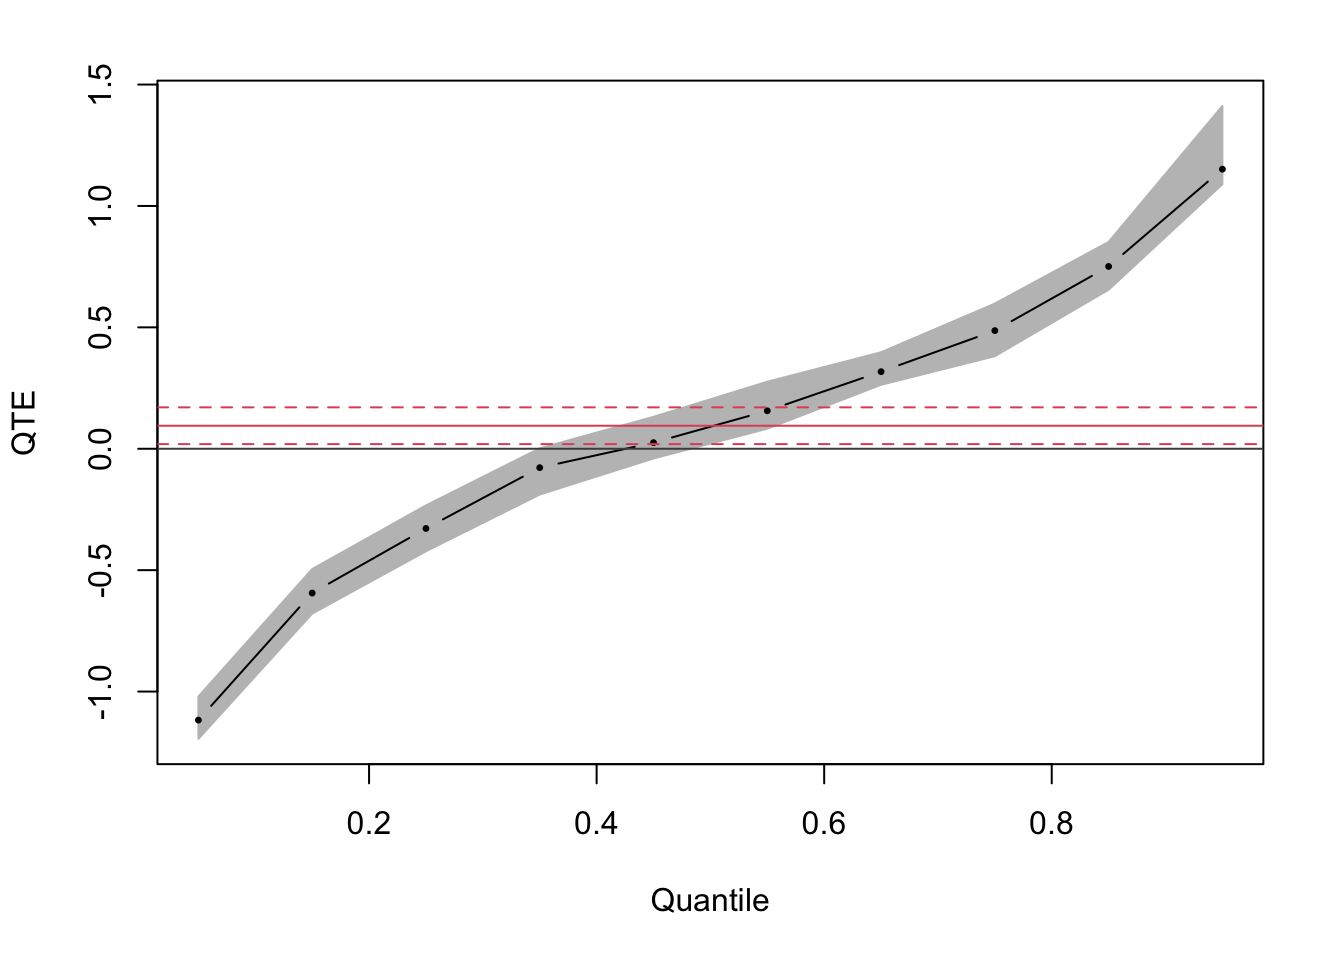
\includegraphics{effect-types_esp_files/figure-latex/unnamed-chunk-6-1.pdf}

\hypertarget{efectos-de-mediaciuxf3n}{%
\section{8 Efectos de mediación}\label{efectos-de-mediaciuxf3n}}

A veces queremos describir no solo la magnitud y el significado de un
efecto causal observado, sino también el mecanismo (o mecanismos) que lo
produjeron. ¿Nuestra intervención aumentó la participación en el grupo
de tratamiento, en parte, porque aumentó el sentido de eficacia política
de estos sujetos? Si es así, ¿cuánto de ese efecto total puede
atribuirse a los efectos mediados por nuestro tratamiento en la eficacia
y de la eficacia en la participación?

Baron y Kenny (1986) ofrecen un marco general para pensar en la
mediación al descomponer el efecto total del tratamiento en su efecto
indirecto sobre un mediador que luego afecta el resultado, llamado
efecto de mediación causal promedio (Average Causal Mediation Effect,
ACME), y el efecto directo promedio restante (emaining Average Direct
Effect, ADE) del tratamiento. Sin embargo, la estimación insesgada de
estos efectos requiere un conjunto de supuestos sólidos sobre la
relación entre el tratamiento, los mediadores, los resultados y los
posibles factores que pueden generar distorsión, denominados
colectivamente ignorabilidad secuencial (Imai, Keele y Yamamoto (2010),
Bullock, Green y Ha (2010). )). \footnote{Imai, Keele y Yamamoto (2010)
  definen formalmente las condiciones necesarias para la ignorabilidad
  secuencial como:
  \({Y_i(d',m),M_i(d)}\perp D_i|X_i=x, Y_i(d',m)\perp M_i(d)|D_i=d,X_i=x\).
  Esto quiere decir, primero, dado unas covariables de pretatamiento,
  los resultados potenciales de Y y M son independientes del tratamiento
  D y segundo que condicionado a las covariables previas al tratamiento
  y al estado del tratamiento, los resultados potenciales también son
  independientes del mediador.}

La mayoría de los efectos causales probablemente operan a través de
múltiples canales, por lo que una suposición de ignorabilidad secuencial
para un experimento puede ser difícil de justificar. Por ejemplo, la
fila superior en la figura siguiente ilustra situaciones en las que se
mantiene la ignorabilidad secuencial, mientras que la fila inferior
muestra dos (de muchos posibles) casos en los que se viola la
ignorabilidad secuencial y el análisis de mediación está sesgado. En
esencia, especificar los efectos de un mediador en particular requiere
suposiciones sólidas sobre el papel de todos los demás mediadores en la
cadena causal. Si bien algunos diseños experimentales pueden, en teoría,
proporcionar un apalancamiento adicional (como ejecutar un segundo
experimento paralelo en el que también se manipula al mediador), en la
práctica estos diseños son difíciles de implementar y sensibles a sesgos
no observados. En algunos casos, los conocimientos que esperamos obtener
del análisis de mediación pueden adquirirse más fácilmente a partir de
análisis de subgrupos y experimentos diseñados para probar la
moderación.

Imai y colegas proponen un enfoque para el análisis de mediación que
permite a los investigadores probar la sensibilidad de sus estimaciones
a violaciones de ignorabilidad secuencial\footnote{Vea por ejemplo Imai,
  Keele, y Yamamoto (2010), Imai et al.~(2011), Imai, Tingley y Yamamoto
  (2013), Imai y Yamamoto (2013). Así como también Imai, Tingley, y
  Yamamoto (2013) para perspectivas diferentes en la desabi for
  different perspectives sobre la conveniencia de abordar hacer
  aserciones sobre posible mediación con análisis de sensibilidad o de
  límites (bounds).}. En el código presentado a continuación mostramos
algunas de las características de este enfoque, implementadas en el
paquete \texttt{mediation} en R (Tingley et al.2014). Modelamos las
relaciones utilizando MCO, pero el paquete es capaz de manejar otros
modelos, como modelos lineales generalizados o modelos aditivos
generales, que pueden ser más apropiados para sus datos. Más importante
aún, el paquete nos permite producir límites que reflejan la
sensibilidad de nuestras estimaciones puntuales a algunas violaciones de
ignorabilidad secuencial. En nuestros datos simulados, poco más del 20
por ciento del efecto total está mediado por nuestro mediador propuesto,
M, y el sesgo de un factor de distorsión previo al tratamiento no
observado tendría que ser bastante grande (\(\rho\) = .7) antes de que
rechacemos el hallazgo de un ACME positivo. Sin embargo, estos límites
solo son válidos si creemos que no hay factores no observados
postratamiento que causen distorsión (como en el panel 4). El análisis
de sensibilidad es posible, pero más complicado en tales entornos (Imai
y Yamamoto 2013).

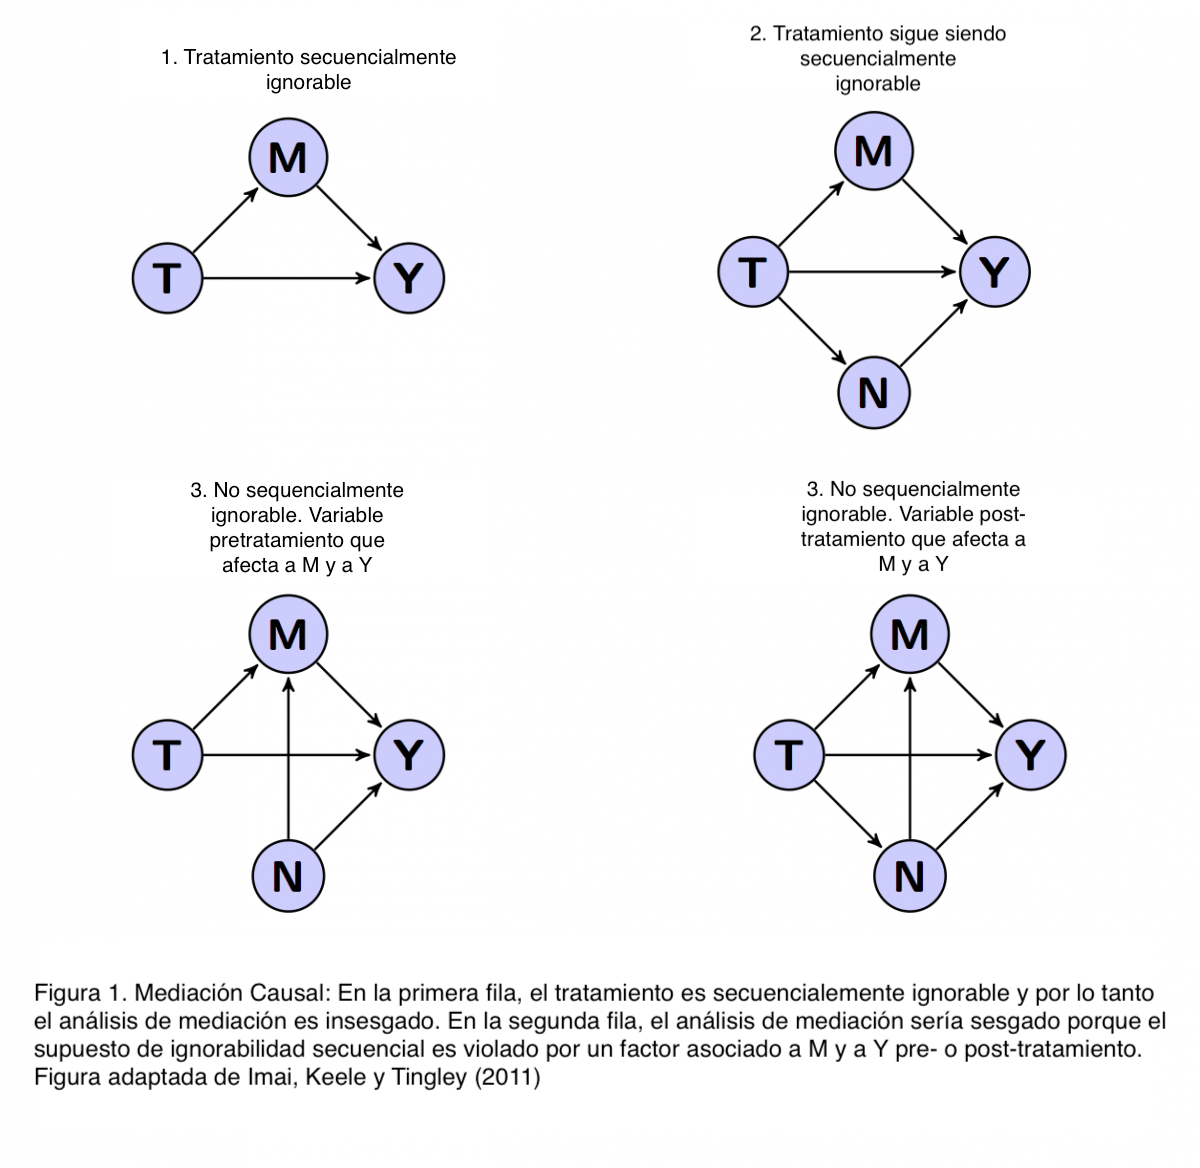
\includegraphics{https://raw.githubusercontent.com/egap/methods-guides/master/effect-types/effect-types_fig2_esp.png}

\begin{Shaded}
\begin{Highlighting}[]
\FunctionTok{set.seed}\NormalTok{(}\DecValTok{1234}\NormalTok{) }\CommentTok{\# Para replicar}
\NormalTok{n }\OtherTok{=} \DecValTok{1000} \CommentTok{\# Tamaño de la muestra}
\NormalTok{Y0 }\OtherTok{=} \FunctionTok{runif}\NormalTok{(n) }\CommentTok{\# Resultado potencial bajo el control}
\NormalTok{D }\OtherTok{=} \FunctionTok{sample}\NormalTok{((}\DecValTok{1}\SpecialCharTok{:}\NormalTok{n)}\SpecialCharTok{\%\%}\DecValTok{2}\NormalTok{) }\CommentTok{\# Tratamiento: 1 si tratado, 0 de lo contrario}
\NormalTok{X}\OtherTok{\textless{}{-}}\FunctionTok{rnorm}\NormalTok{(n) }\CommentTok{\# Covariables}
\NormalTok{M}\OtherTok{\textless{}{-}}\FunctionTok{rnorm}\NormalTok{(}\AttributeTok{n=}\NormalTok{n,}\AttributeTok{mean=}\NormalTok{D}\SpecialCharTok{+}\FunctionTok{rnorm}\NormalTok{(n)) }\CommentTok{\# Mediador influenciado por el tratamiento}
\NormalTok{Y1 }\OtherTok{=}\NormalTok{ Y0 }\SpecialCharTok{+} \DecValTok{1} \SpecialCharTok{+}\NormalTok{ M }\CommentTok{\#  Resultado potencial bajo el tratamiento}
\NormalTok{Y }\OtherTok{=}\NormalTok{ D}\SpecialCharTok{*}\NormalTok{Y1 }\SpecialCharTok{+}\NormalTok{ (}\DecValTok{1}\SpecialCharTok{{-}}\NormalTok{D)}\SpecialCharTok{*}\NormalTok{Y0 }\CommentTok{\#  Variable de resultado de la población }
\NormalTok{samp}\OtherTok{\textless{}{-}}\FunctionTok{data.frame}\NormalTok{(D,M,Y) }

\FunctionTok{library}\NormalTok{(mediation) }
\NormalTok{med.f}\OtherTok{\textless{}{-}}\FunctionTok{lm}\NormalTok{(M}\SpecialCharTok{\textasciitilde{}}\NormalTok{D}\SpecialCharTok{+}\NormalTok{X,}\AttributeTok{data=}\NormalTok{samp) }\CommentTok{\# Modelo para el mediador}
\NormalTok{out.f}\OtherTok{\textless{}{-}}\FunctionTok{lm}\NormalTok{(Y}\SpecialCharTok{\textasciitilde{}}\NormalTok{M}\SpecialCharTok{+}\NormalTok{D}\SpecialCharTok{+}\NormalTok{X,}\AttributeTok{data=}\NormalTok{samp) }\CommentTok{\# Modelo para la variable de resultado}

\CommentTok{\#Estimado del ACME y el  ADE }
\FunctionTok{library}\NormalTok{(mediation) }
\NormalTok{med.out}\OtherTok{\textless{}{-}}
\FunctionTok{mediate}\NormalTok{(med.f,out.f,}\AttributeTok{treat=}\StringTok{"D"}\NormalTok{,}\AttributeTok{mediator=}\StringTok{"M"}\NormalTok{,}\AttributeTok{robustSE=}\NormalTok{T,}\AttributeTok{sims=}\DecValTok{1000}\NormalTok{) }
\CommentTok{\# Sensibilidad del ACME a variables que no observadas que }
\CommentTok{\# pueden generar distorsión}
\NormalTok{s.out}\OtherTok{\textless{}{-}}\FunctionTok{medsens}\NormalTok{(med.out) }

\FunctionTok{plot}\NormalTok{(s.out) }\CommentTok{\# Grafica limites de sensibilidad}
\end{Highlighting}
\end{Shaded}

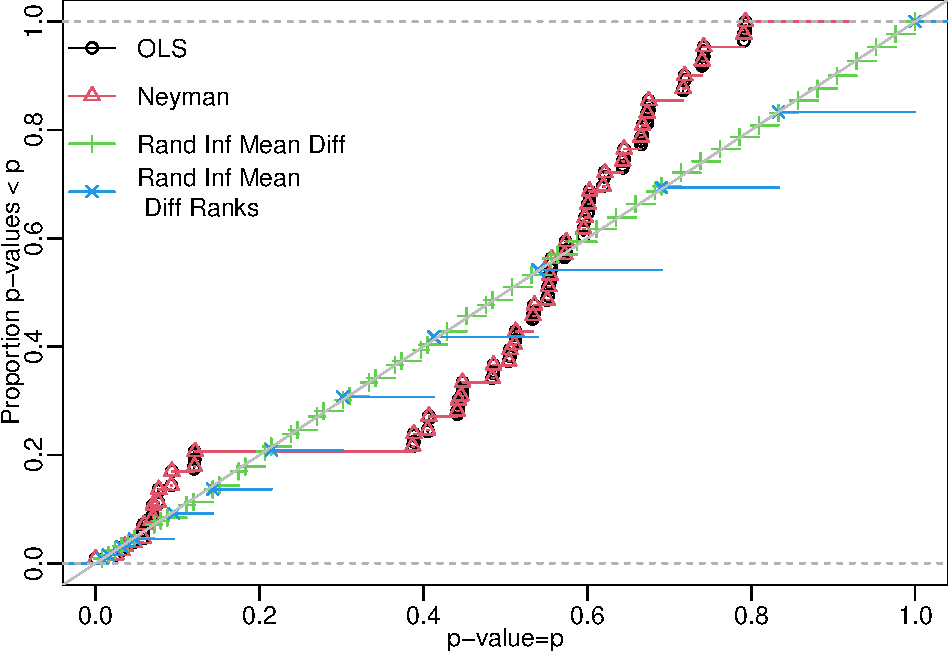
\includegraphics{effect-types_esp_files/figure-latex/unnamed-chunk-7-1.pdf}

\hypertarget{efectos-del-tratamiento-con-probabilidades-logaruxedtmicas}{%
\section{9 Efectos del tratamiento con probabilidades
logarítmicas}\label{efectos-del-tratamiento-con-probabilidades-logaruxedtmicas}}

Los efectos promedio del tratamiento parecen un poco difíciles de
interpretar cuando los resultados no son continuos. Por ejemplo, un
resultado binario muy común en el estudio de las elecciones se codifica
como 1 cuando los sujetos votaron y 0 cuando no lo hicieron. El efecto
promedio podría ser 0.2, pero ¿qué significa realmente decir que un
tratamiento aumentó mi voto en 0.2? La estimación de los efectos
causales de los resultados dicotómicos requiere un cuidado adicional, en
particular cuando se incluyen covariables. Una cantidad común de interés
causal para los resultados dicotómicos es el efecto de nuestro
tratamiento sobre las probabilidades de éxito logarítmicas, definidas
para el grupo experimental como:

\[\Delta = log\frac{E(Y_i(1))}{1-E(Y_i(1))} - log\frac{E(Y_i(0))}{1-E(Y_i(0))}\]
Freedman (2008b) muestra que la regresión logística ajustada por
covariables en experimentos aleatorios produce estimaciones sesgadas de
este efecto causal. La intuición básica del argumento de Freedman
proviene del hecho de que tomar el logaritmo de promedios no es lo mismo
que tomar el promedio de logaritmos y, por lo tanto, el coeficiente de
tratamiento estimado a partir de un condicionamiento de regresión
logística sobre covariables no proporcionará un estimador consistente de
probabilidades logarítmicas de éxito. Freedman recomienda en cambio
tomar las probabilidades pronosticadas que varían el estado de
tratamiento de los sujetos, pero manteniendo sus perfiles de covariables
observados para producir un estimador consistente de las probabilidades
logarítmicas.

El procedimiento básico se describe en el código presentado a
continuación. Los coeficientes de la regresión logística que controlan
la covariable X tienden a sobrestimar el efecto del tratamiento en las
probabilidades logarítmicas, mientras que las estimaciones ajustadas de
las probabilidades predecidas producen resultados consistentes.

\begin{Shaded}
\begin{Highlighting}[]
\FunctionTok{set.seed}\NormalTok{(}\DecValTok{1234}\NormalTok{) }\CommentTok{\# Para replicar }
\NormalTok{n }\OtherTok{=} \DecValTok{1000} \CommentTok{\# Tamaño de muestra}
\NormalTok{U }\OtherTok{=} \FunctionTok{runif}\NormalTok{(n) }
\NormalTok{X }\OtherTok{=} \FunctionTok{runif}\NormalTok{(n) }\CommentTok{\# Covariables obsersvadas}
\NormalTok{Y0 }\OtherTok{=} \FunctionTok{ifelse}\NormalTok{(U}\SpecialCharTok{\textgreater{}}\NormalTok{.}\DecValTok{5}\NormalTok{,}\DecValTok{1}\NormalTok{,}\DecValTok{0}\NormalTok{) }\CommentTok{\# Resultados potenciales}
\NormalTok{Y1 }\OtherTok{=} \FunctionTok{ifelse}\NormalTok{(U}\SpecialCharTok{+}\NormalTok{X}\SpecialCharTok{\textgreater{}}\NormalTok{.}\DecValTok{75}\NormalTok{,}\DecValTok{1}\NormalTok{,}\DecValTok{0}\NormalTok{) }
\NormalTok{D }\OtherTok{=} \FunctionTok{rbinom}\NormalTok{(n,}\DecValTok{1}\NormalTok{,.}\DecValTok{75}\NormalTok{) }\CommentTok{\# Asignar aleatoriamente 3/4 al tratamiento }
\NormalTok{Y }\OtherTok{=}\NormalTok{ D}\SpecialCharTok{*}\NormalTok{Y1}\SpecialCharTok{+}\NormalTok{Y0}\SpecialCharTok{*}\NormalTok{(}\DecValTok{1}\SpecialCharTok{{-}}\NormalTok{D) }
\NormalTok{samp }\OtherTok{=} \FunctionTok{data.frame}\NormalTok{(X,D,Y) }
\NormalTok{aT}\OtherTok{\textless{}{-}}\FunctionTok{with}\NormalTok{(samp, }\FunctionTok{mean}\NormalTok{(Y[D}\SpecialCharTok{==}\DecValTok{1}\NormalTok{])) }
\NormalTok{aC}\OtherTok{\textless{}{-}}\FunctionTok{with}\NormalTok{(samp, }\FunctionTok{mean}\NormalTok{(Y[D}\SpecialCharTok{==}\DecValTok{0}\NormalTok{])) }

\CommentTok{\# log odds incondicional}
\NormalTok{log.odds}\OtherTok{\textless{}{-}}\FunctionTok{log}\NormalTok{(aT}\SpecialCharTok{/}\NormalTok{(}\DecValTok{1}\SpecialCharTok{{-}}\NormalTok{aT))}\SpecialCharTok{{-}}\FunctionTok{log}\NormalTok{(aC}\SpecialCharTok{/}\NormalTok{(}\DecValTok{1}\SpecialCharTok{{-}}\NormalTok{aC)) }

\CommentTok{\# Regresión logística condicionando en X estima el log odds por encima}
\NormalTok{fit}\OtherTok{\textless{}{-}}\FunctionTok{glm}\NormalTok{(Y}\SpecialCharTok{\textasciitilde{}}\NormalTok{D}\SpecialCharTok{+}\NormalTok{X,}\AttributeTok{data=}\NormalTok{samp,}\FunctionTok{binomial}\NormalTok{(}\StringTok{"logit"}\NormalTok{)) }
\NormalTok{log.odds.logit}\OtherTok{\textless{}{-}}
  \FunctionTok{coef}\NormalTok{(}\FunctionTok{glm}\NormalTok{(Y}\SpecialCharTok{\textasciitilde{}}\NormalTok{D}\SpecialCharTok{+}\NormalTok{X,}\AttributeTok{data=}\NormalTok{samp,}\FunctionTok{binomial}\NormalTok{(}\StringTok{"logit"}\NormalTok{)))[}\DecValTok{2}\NormalTok{] }

\CommentTok{\# Dataframes tilizando covariables originales para las probabilidades de predicción}
\NormalTok{D1}\OtherTok{\textless{}{-}}\FunctionTok{data.frame}\NormalTok{(}\AttributeTok{D=}\DecValTok{1}\NormalTok{,samp[,}\FunctionTok{c}\NormalTok{(}\StringTok{"X"}\NormalTok{)]) }
\NormalTok{D0}\OtherTok{\textless{}{-}}\FunctionTok{data.frame}\NormalTok{(}\AttributeTok{D=}\DecValTok{0}\NormalTok{,samp[,}\FunctionTok{c}\NormalTok{(}\StringTok{"X"}\NormalTok{)]) }
\CommentTok{\# log{-}odds ajustado produce un estimador consistente del log{-}odds }
\NormalTok{aT.adj}\OtherTok{\textless{}{-}}\FunctionTok{predict}\NormalTok{(fit,}\AttributeTok{newdata=}\NormalTok{D1,}\AttributeTok{type=}\StringTok{"response"}\NormalTok{) }
\NormalTok{aC.adj}\OtherTok{\textless{}{-}}\FunctionTok{predict}\NormalTok{(fit,}\AttributeTok{newdata=}\NormalTok{D0,}\AttributeTok{type=}\StringTok{"response"}\NormalTok{) }
\NormalTok{log.odds.adj}\OtherTok{\textless{}{-}}\FunctionTok{log}\NormalTok{(}\FunctionTok{mean}\NormalTok{(aT.adj)}\SpecialCharTok{/}\NormalTok{(}\DecValTok{1}\SpecialCharTok{{-}}\FunctionTok{mean}\NormalTok{(aT.adj)))}\SpecialCharTok{{-}}
  \FunctionTok{log}\NormalTok{(}\FunctionTok{mean}\NormalTok{(aC.adj)}\SpecialCharTok{/}\NormalTok{(}\DecValTok{1}\SpecialCharTok{{-}}\FunctionTok{mean}\NormalTok{(aC.adj)))}
\end{Highlighting}
\end{Shaded}

\hypertarget{efectos-atribuibles}{%
\section{10 Efectos atribuibles}\label{efectos-atribuibles}}

Concluimos con una breve discusión de una cantidad alternativa de
interés causal que puede ser particularmente útil con resultados
binarios: el efecto atribuible (Rosenbaum 2010). Considere un caso
simple con un resultado y un tratamiento dicotómicos. Sea \(A\) el
número de resultados atribuibles al tratamiento, es decir, el número de
casos en los que \(Y_i\) es igual a 1 entre los sujetos tratados y que
de haber sido asginados al control no habrían producido el mismo
resultado. Para un rango de \(A\), ajustamos la tabla de contingencia
observada de resultados entre las unidades tratadas y comparamos esta
distribución resultante con una distribución nula conocida (la
distribución de resultados que hubiéramos observado si el tratamiento no
hubiera tenido efecto). El rango resultante de \(A\) para el cual
nuestra prueba continúa rechazando la hipótesis nula de ningún efecto
proporciona un rango de efectos que son atribuibles a nuestro
tratamiento.

Tabla 1\textbar{}\(D=1\) \textbar{}\(D=0\)
-------\textbar-------------------\textbar-------------- \(Y=1\)
\textbar{}\(\sum Y_iD_i-A\) \textbar{}\((1-Y_i)(D_i)\) \(Y=0\)
\textbar{}\(\sum Y_i(1-D_i)+A\)\textbar{}\(\sum (1-Y_i)(1-D_i)\)

Rosenbaum (2002) presenta extensiones de este concepto para diferentes
tipos de resultados (como las variables continuas). Se puede aplicar una
lógica similar para detectar respuestas poco comunes al tratamiento,
pero extremas (Rosenbaum y Silber 2008).

Hansen y Bowers (2009) utilizan este enfoque para identificar el número
de votos adicionales atribuibles a diferentes intervenciones en un
experimento para incentivar el voto con asignación al tratamiento por
conglomerados e incumplimiento unilateral. Ellos muestran que en
muestras grandes se puede aproximar el intervalo de confianza para los
efectos atribuibles sin evaluar cada atribución. A continuación
presentamos un ejemplo de ese enfoque en el que se utilizan covariables
para aumentar la precisión.

En primer lugar, definimos un efecto atribuible como
\(A=\sum_iZ_i\tau_i\), donde \(\tau_i=Y_i(1)-Y_i(0)\) y \(y\in0,1\) como
se muestra en Rosenbaum (2002). Es decir, el efecto atribuible es el
número de ``sis'' o ``exitos'' o otras respuestas de ``1'' entre las
unidades tratadas que no hubieramos obtenido si estas unidades hubieran
sido asignadas al grupo de control.

En segundo lugar, como puede darse cuenta si escribimos el set \(U\)
como el universo experimental, y el set de unidades en el grupo de
control es un subconjuto de este universo, \(C\subseteq U\), por lo
tanto podemos decir que \(\sum_{i\in C}Y_i-Y_i(0)=0\). Esto quiere decir
que podemos representar \(A\) utulizando totales:
\[A = \sum_{i=1}^NZ_i\tau_i=\sum_{i=1}^NZ_i(Y_i(1)-Y_i(0))=\sum_{i\notin C}y_i(1)-sum_{i\notin C}y_i(0)\]

\[  = \sum_{i\notin C}Y_i-\sum_{i\notin C}Y_i(0)=\sum_{i=1}^NY_i-\sum_{i=1}^NY_i(0)=t_U-t_C\]

= total observado general (fijo y observado) - total variable de
resultado cuando es asignada al grupo de control (no observado, para
estimar)

En tercer lugar, esta representación nos permite producir un intervalo
de confianza basado en el diseño para A\^{} basándonos en la literatura
de muestreo de encuestas sobre inferencia estadística para totales de
muestra porque los resultados totales observados, tU, se fijan en las
aleatorizaciones. Podemos usar covariables para aumentar la precisión
aquí porque el estimador de regresión de la encuesta nos permite estimar
el total que habríamos visto en el grupo de control:
\(\hat{t}_c=\sum_{i\in U}\hat{Y}_i+\sum_{i\in U}(Y_i-\hat{Y}_i)\) with
\(\hat{Y}_i=f(X_i,\beta)\) (Lohr 1999). La literatura the muestreo de
encuestas prueba que a medida que \(N\rightarrow \infty\),
\(CI(\hat{t}_c) \approx \hat{t}_c \pm z_{a/2}SE(\hat{t}_c)\). Por lo que
se puede calcular \(\widehat{SE}(\hat{t}_c)\) de acuerdo a la teoría
estándar de muestreo y luego el
\(CI(\hat{A}) \approx t_U-\widehat{CI}(\hat{t}_c)\).

En el siguiente código, proporcionamos una ilustración que utiliza datos
simulados para una respuesta y un tratamiento binarios. En el 85 por
ciento del grupo de tratamiento, \(Y = 1\) en comparación con el 52 por
ciento en el grupo de control. Una diferencia de este tamaño es
consistente con que nuestro tratamiento fue la causa de que \(Y = 1\)
para entre 92 y 138 sujetos, para quienes \(Y\) habría sido igual a 0 si
no hubieran recibido el tratamiento. El estimador de regresión, que
aprovecha la precisión obtenida al incluir covariables, produce
intervalos de confianza más estrictos (98,8 a 135,1) para los efectos
atribuibles.

\begin{Shaded}
\begin{Highlighting}[]
\FunctionTok{set.seed}\NormalTok{(}\DecValTok{1234}\NormalTok{) }\CommentTok{\# Para replicar }
\NormalTok{n }\OtherTok{=} \DecValTok{1000} \CommentTok{\# Tamaño de la muestra}
\NormalTok{X1 }\OtherTok{=} \FunctionTok{rnorm}\NormalTok{(n) }\CommentTok{\# Covariables}
\NormalTok{X2 }\OtherTok{=} \FunctionTok{rnorm}\NormalTok{(n) }
\NormalTok{p }\OtherTok{=} \FunctionTok{pnorm}\NormalTok{(}\SpecialCharTok{{-}}\FloatTok{0.5} \SpecialCharTok{+} \FloatTok{0.75}\SpecialCharTok{*}\NormalTok{X2) }\CommentTok{\# Probabilidad desigual }
                           \CommentTok{\# de asignación al tratamiento }
\NormalTok{D }\OtherTok{=} \FunctionTok{rbinom}\NormalTok{(n, }\DecValTok{1}\NormalTok{, p) }
\NormalTok{p0 }\OtherTok{=} \FunctionTok{pnorm}\NormalTok{(}\FunctionTok{rnorm}\NormalTok{(n)) }\CommentTok{\# Resultados potenciales para variable binaria}
\NormalTok{p1 }\OtherTok{=} \FunctionTok{pnorm}\NormalTok{(X1 }\SpecialCharTok{+}\NormalTok{ X2}\SpecialCharTok{+}\DecValTok{1}\NormalTok{) }
\NormalTok{Y0 }\OtherTok{=} \FunctionTok{rbinom}\NormalTok{(n, }\DecValTok{1}\NormalTok{, p0) }
\NormalTok{Y1 }\OtherTok{=} \FunctionTok{rbinom}\NormalTok{(n, }\DecValTok{1}\NormalTok{, p1) }
\NormalTok{Y }\OtherTok{=}\NormalTok{ D}\SpecialCharTok{*}\NormalTok{Y1 }\SpecialCharTok{+}\NormalTok{ (}\DecValTok{1}\SpecialCharTok{{-}}\NormalTok{D)}\SpecialCharTok{*}\NormalTok{Y0 }\CommentTok{\#  Variable de resultado observada}
\NormalTok{samp }\OtherTok{=} \FunctionTok{data.frame}\NormalTok{(D,Y,X1,X2) }\CommentTok{\# Base de datos}

\NormalTok{attribute}\OtherTok{\textless{}{-}}\ControlFlowTok{function}\NormalTok{(treat,out,A,data)\{ }
  \CommentTok{\# Tabla de contigencia del estado del tratamiento}
  \CommentTok{\# y la variable de resultado }
\NormalTok{  attr.tab}\OtherTok{\textless{}{-}}\FunctionTok{with}\NormalTok{(data,}\FunctionTok{table}\NormalTok{(treat,out)) }\CommentTok{\# }
  \CommentTok{\# Matriz de valores p para efectos atribuibles A}
\NormalTok{  attr.ps}\OtherTok{\textless{}{-}}
    \FunctionTok{matrix}\NormalTok{(}\ConstantTok{NA}\NormalTok{,}\AttributeTok{nc=}\DecValTok{2}\NormalTok{,}\AttributeTok{nr=}\NormalTok{A,}\AttributeTok{dimnames=}\FunctionTok{list}\NormalTok{(}\ConstantTok{NULL}\NormalTok{,}\FunctionTok{c}\NormalTok{(}\StringTok{"A"}\NormalTok{,}\StringTok{"p"}\NormalTok{))) }
  \ControlFlowTok{for}\NormalTok{(i }\ControlFlowTok{in} \DecValTok{1}\SpecialCharTok{:}\NormalTok{A)\{ }
\NormalTok{    attr.ps[i,]}\OtherTok{\textless{}{-}}
      \FunctionTok{c}\NormalTok{(i,}\FunctionTok{fisher.test}\NormalTok{(attr.tab}\SpecialCharTok{+}\FunctionTok{matrix}\NormalTok{(}\FunctionTok{c}\NormalTok{(}\DecValTok{0}\NormalTok{,i,}\DecValTok{0}\NormalTok{,}\SpecialCharTok{{-}}\NormalTok{i),}\DecValTok{2}\NormalTok{,}\DecValTok{2}\NormalTok{))}\SpecialCharTok{$}\NormalTok{p) }
\NormalTok{    \}}
  \CommentTok{\# Determina el rango de los efectos}
\NormalTok{  get.bounds}\OtherTok{\textless{}{-}}\ControlFlowTok{function}\NormalTok{()\{ }
\NormalTok{    diffs}\OtherTok{\textless{}{-}}\FunctionTok{ifelse}\NormalTok{(.}\DecValTok{05}\SpecialCharTok{{-}}\NormalTok{attr.ps[,}\StringTok{"p"}\NormalTok{]}\SpecialCharTok{\textgreater{}}\DecValTok{0}\NormalTok{,.}\DecValTok{05}\SpecialCharTok{{-}}
\NormalTok{                    attr.ps[,}\StringTok{"p"}\NormalTok{],}\DecValTok{99}\NormalTok{) }
\NormalTok{    index}\OtherTok{\textless{}{-}}\NormalTok{(diffs }\SpecialCharTok{\%in\%} 
              \FunctionTok{c}\NormalTok{(}\FunctionTok{min}\NormalTok{(diffs),}\FunctionTok{min}\NormalTok{(diffs[diffs}\SpecialCharTok{\textgreater{}}\FunctionTok{min}\NormalTok{(diffs)]))) }
\NormalTok{    index }
\NormalTok{    \}}
  \CommentTok{\# Devuelve el rango de los efectos}
  \FunctionTok{return}\NormalTok{ (attr.ps[}\FunctionTok{get.bounds}\NormalTok{(),])}
\NormalTok{  \} }
\FunctionTok{with}\NormalTok{(samp,}\FunctionTok{table}\NormalTok{(D,Y))}
\end{Highlighting}
\end{Shaded}

\begin{verbatim}
##    Y
## D     0   1
##   0 318 339
##   1  51 292
\end{verbatim}

\begin{Shaded}
\begin{Highlighting}[]
\FunctionTok{with}\NormalTok{(samp,}\FunctionTok{apply}\NormalTok{(}\FunctionTok{table}\NormalTok{(D,Y),}\DecValTok{1}\NormalTok{,prop.table)) }
\end{Highlighting}
\end{Shaded}

\begin{verbatim}
##    D
## Y           0        1
##   0 0.4840183 0.148688
##   1 0.5159817 0.851312
\end{verbatim}

\begin{Shaded}
\begin{Highlighting}[]
\FunctionTok{attribute}\NormalTok{(}\AttributeTok{treat =}\NormalTok{ D, }\AttributeTok{out=}\NormalTok{ Y, }\AttributeTok{A=}\DecValTok{200}\NormalTok{,}\AttributeTok{data=}\NormalTok{samp) }
\end{Highlighting}
\end{Shaded}

\begin{verbatim}
##        A          p
## [1,]  92 0.04519869
## [2,] 138 0.04587804
\end{verbatim}

\begin{Shaded}
\begin{Highlighting}[]
\CommentTok{\# Estimador de la regresión}
\NormalTok{fit1}\OtherTok{\textless{}{-}}\FunctionTok{lm}\NormalTok{(Y}\SpecialCharTok{\textasciitilde{}}\NormalTok{X1}\SpecialCharTok{+}\NormalTok{X2,}\AttributeTok{data=}\NormalTok{samp,}\AttributeTok{subset=}\NormalTok{D}\SpecialCharTok{==}\DecValTok{0}\NormalTok{) }
\NormalTok{hatYcU}\OtherTok{\textless{}{-}}\FunctionTok{predict}\NormalTok{(fit1,}\AttributeTok{newdata=}\NormalTok{samp) }
\NormalTok{ec}\OtherTok{\textless{}{-}}\NormalTok{Y[D}\SpecialCharTok{==}\DecValTok{0}\NormalTok{]}\SpecialCharTok{{-}}\NormalTok{hatYcU[D}\SpecialCharTok{==}\DecValTok{0}\NormalTok{] }\DocumentationTok{\#\# lo mismo que residuals(fit1) }
\NormalTok{hatTotYc}\OtherTok{\textless{}{-}}\FunctionTok{sum}\NormalTok{(hatYcU)}\SpecialCharTok{+}\FunctionTok{sum}\NormalTok{(ec) }
\NormalTok{N}\OtherTok{\textless{}{-}}\FunctionTok{length}\NormalTok{(Y) }
\NormalTok{nctrls}\OtherTok{\textless{}{-}}\FunctionTok{sum}\NormalTok{(}\DecValTok{1}\SpecialCharTok{{-}}\NormalTok{D) }
\NormalTok{thefpc}\OtherTok{\textless{}{-}}\NormalTok{ (}\DecValTok{1} \SpecialCharTok{{-}}\NormalTok{ (nctrls}\SpecialCharTok{/}\NormalTok{N)) }
\NormalTok{varhattC}\OtherTok{\textless{}{-}}\NormalTok{N}\SpecialCharTok{*}\NormalTok{thefpc}\SpecialCharTok{*}\FunctionTok{var}\NormalTok{(Y[D}\SpecialCharTok{==}\DecValTok{0}\NormalTok{]) }
\NormalTok{alpha}\OtherTok{\textless{}{-}}\FunctionTok{c}\NormalTok{(.}\DecValTok{05}\NormalTok{, }\DecValTok{1}\SpecialCharTok{/}\DecValTok{3}\NormalTok{) }
\NormalTok{alpha}\OtherTok{\textless{}{-}}\FunctionTok{sort}\NormalTok{(}\FunctionTok{c}\NormalTok{(alpha}\SpecialCharTok{/}\DecValTok{2}\NormalTok{, }\DecValTok{1}\SpecialCharTok{{-}}\NormalTok{alpha}\SpecialCharTok{/}\DecValTok{2}\NormalTok{)) }
\NormalTok{ciTotYc}\OtherTok{\textless{}{-}}\NormalTok{hatTotYc}\SpecialCharTok{+}\FunctionTok{sqrt}\NormalTok{(varhattC)}\SpecialCharTok{*}\FunctionTok{qnorm}\NormalTok{(alpha) }
\NormalTok{ciAE}\OtherTok{\textless{}{-}}\FunctionTok{sort}\NormalTok{(}\FunctionTok{sum}\NormalTok{(Y) }\SpecialCharTok{{-}}\NormalTok{ ciTotYc ) }
\FunctionTok{names}\NormalTok{(ciAE)}\OtherTok{\textless{}{-}}\FunctionTok{c}\NormalTok{(}\StringTok{"limite bajo 95\%"}\NormalTok{,}\StringTok{"limite bajo }
\StringTok{66\%"}\NormalTok{,}\StringTok{"limite alto 66\%"}\NormalTok{,}\StringTok{"llimite alto 95\%"}\NormalTok{) }
\FunctionTok{print}\NormalTok{(ciAE) }
\end{Highlighting}
\end{Shaded}

\begin{verbatim}
##   limite bajo 95% limite bajo \n66%   limite alto 66%  llimite alto 95% 
##          98.78637         107.97975         125.90114         135.09451
\end{verbatim}

\hypertarget{referencias}{%
\section{Referencias}\label{referencias}}

Aronow, Peter M, y Joel A Middleton. 2013. ``A Class of Unbiased
Estimators of the Average Treatment Effect in Randomized Experiments.''
Journal of Causal Inference 1 (1): 135--54.

Aronow, Peter M, y Cyrus Samii. 2014. ``Does Regression Produce
Representative Estimates of Causal Effects?'' In EPSA 2013 Annual
General Conference Paper. Vol. 585.

Baron, Reuben M, y David A Kenny. 1986. ``The Moderator--Mediator
Variable Distinction in Social Psychological Research: Conceptual,
Strategic, and Statistical Considerations.'' Journal of Personality and
Social Psychology 51 (6). American Psychological Association: 1173.

Bound, John, David A Jaeger, y Regina M Baker. 1995. ``Problems with
Instrumental Variables Estimation When the Correlation Between the
Instruments and the Endogenous Explanatory Variable Is Weak.'' Journal
of the American Statistical Association 90 (430). Taylor \& Francis:
443--50.

Brambor, Thomas, William R. Clark, y Matt Golder. 2006. ``Understanding
Interaction Models: Improving Empirical Analyses.'' Political Analysis
14 (1): 63--82.

Bullock, John G, Donald P Green, y Shang E Ha. 2010. ``Yes, but What's
the Mechanism?(don't Expect an Easy Answer).'' Journal of Personality
and Social Psychology 98 (4). American Psychological Association: 550.

Chernozhukov, Victor, y Christian Hansen. 2005. ``An IV Model of
Quantile Treatment Effects.'' Econometrica 73 (1). Wiley Online Library:
245--61.

Dunning, Thad. 2010. ``Design-Based Inference: Beyond the Pitfalls of
Regression Analysis?'' Rethinking Social Inquiry: Diverse Tools, Shared
Standards. 2nd Ed. Lanham, Md.: Rowman and Littlefield.

Freedman, David A. 2008a. ``On Regression Adjustments to Experimental
Data.'' Advances in Applied Mathematics 40 (2). Elsevier: 180--93.
---------. 2008b. ``Randomization Does Not Justify Logistic
Regression.'' Statistical Science 23 (2). Institute of Mathematical
Statistics: 237--49.

Frölich, Markus, y Blaise Melly. 2010. ``Estimation of Quantile
Treatment Effects with Stata.'' Stata Journal 10 (3): 423.

Gerber, Alan S, y Donald P Green. 2012. Field Experiments: Design,
Analysis, and Interpretation. WW Norton.

Green, Donald P. 2009. ``Regression Adjustments to Experimental Data: Do
David Freedman's Concerns Apply to Political Science?'' In 26th Annual
Meeting of the Society for Political Methodology, Yale University, July,
23--25.

Hansen, Ben, y Jake Bowers. 2009. ``Attributing Effects to a
Cluster-Randomized Get-Out-the-Vote Campaign.'' Journal of the American
Statistical Association 104 (487). Taylor \& Francis: 873--85.

Hartman, Erin, RD Grieve, R Ramsahai, and Jasjeet S Sekhon. forthcoming.
``From SATE to PATT: Combining Experimental with Observational
Studies.'' Journal of the Royal Statistical Society.

Hirano, Keisuke, Guido W Imbens, y Geert Ridder. 2003. ``Efficient
Estimation of Average Treatment Effects Using the Estimated Propensity
Score.'' Econometrica 71 (4). Wiley Online Library: 1161--89.

Holland, Paul W. 1986. ``Statistics and Causal Inference.'' Journal of
the American Statistical Association 81 (396). Taylor \& Francis:
945--60.

Imai, K., L. Keele, D. Tingley, y T. Yamamoto. 2011. ``Unpacking the
Black Box of Causality: Learning About Causal Mechanisms from
Experimental and Observational Studies.'' American Political Science
Review 105 (4). Cambridge Univ Press: 765--89.

Imai, Kosuke, y Teppei Yamamoto. 2013. ``Identification and Sensitivity
Analysis for Multiple Causal Mechanisms: Revisiting Evidence from
Framing Experiments.'' Political Analysis 21 (2). SPM-PMSAPSA: 141--71.

Imai, Kosuke, Luke Keele, y Teppei Yamamoto. 2010. ``Identification,
Inference and Sensitivity Analysis for Causal Mediation Effects.''
Statistical Science. JSTOR, 51--71.

Imai, Kosuke, Gary King, and Elizabeth A Stuart. 2008.
``Misunderstandings Between Experimentalists and Observationalists About
Causal Inference.'' Journal of the Royal Statistical Society: series A
(Statistics in Society) 171 (2). Wiley Online Library: 481--502.

Imai, Kosuke, Dustin Tingley, and Teppei Yamamoto. 2013. ``Experimental
Designs for Identifying Causal Mechanisms.'' Journal of the Royal
Statistical Society: Series A (Statistics in Society) 176 (1). Wiley
Online Library: 5--51.

Lin, Winston. 2013. ``Agnostic Notes on Regression Adjustments to
Experimental Data: Reexamining Freedman's Critique.'' The Annals of
Applied Statistics 7 (1). Institute of Mathematical Statistics:
295--318.

Lohr, Sharon L. 1999. ``Sampling: DesignandAnalysis.'' Pacific Grove,
CA: Brooks/Cole.

Neyman, Jerzy. 1990 {[}1923{]}. ``On the Application of Probability
Theory to Agricultural Experiments. Essay on Principles. Section 9.''
Statistical Science 5 (4). Institute of Mathematical Statistics: 465--72
(Translated by D.M. Dabrowska and T.P. Speed from the original Polish).

Nickerson, D.W. 2008. ``Is Voting Contagious? Evidence from Two Field
Experiments.'' American Political Science Review 102 (1). Cambridge Univ
Press: 49.

Rosenbaum, Paul. 2002. ``Attributing Effects to Treatment in Matched
Observational Studies.'' Journal of the American Statistical Association
97 (457). Taylor \& Francis: 183--92.

Rosenbaum, Paul R. 2002. Observational Studies. Springer.

Rosenbaum, Paul, and Donald B. Rubin. 1983. ``The Central Role of the
Propensity Score in Observational Studies for Causal Effects.''
Biometrika 70 (1). Biometrika Trust: 41--55.

Rosenbaum, Paul, and Jeffrey H Silber. 2008. ``Aberrant Effects of
Treatment.'' Journal of the American Statistical Association 103 (481).
Taylor \& Francis: 240--47.

Rosenbaum, PR. 2010. ``Design of Observational Studies.'' Springer
Series in Statistics. New York {[}etc.{]}: Springer. Tingley, Dustin,
Teppei Yamamoto, Kentaro Hirose, Luke Keele, and Kosuke Imai. 2014.
``mediation: R Package for Causal Mediation Analysis.'' Journal of
Statistical Software 59 (5): 1--38.
\url{http://www.jstatsoft.org/v59/i05/}.

\end{document}
